\section{Importance Sampling}
\label{sec:importance_sampling}
Importance sampling is a simulation technique that allows us to approximate integrals w.r.t a measure of interest, the target, by sampling from a tractable approximation, the proposal, instead, thus performing Monte-Carlo integration. To account for the fact that we did not sample from the correct probability measure, we weight samples according to their importance. As the user has freedom in the choice of approximation (except for some technical conditions), importance sampling also acts as a variance reduction technique with better approximations resulting in smaller Monte-Carlo variance. Thus the role that importance sampling plays is twofold: first, it enables Monte-Carlo integration even if sampling from the target is not possible, and second it allows us to do so in an efficient way by choosing, to be defined precisely below, the approximation in an optimal way.

Alternative approaches to importance sampling for performing inference in \glspl{ssm} include \gls{mcmc} and \gls{smc}. 
Recall from the introduction to this chapter that this inference concerns three objectives: maximum likelihood estimation, i.e. evaluation and optimization of the likelihood, access to the posterior distribution $X_{:n} | Y_{:n}$ and prediction of future states and observations. Let us give a concise comparison of these alternative approaches, weighing their advantages and disadvantages over importance sampling, in particular for the \glspl{ssm} that this thesis deals with. 

% MCMC intro
\gls{mcmc} \citep{Brooks2011Handbook} is a simulation technique that allows to simulation of correlated samples from a target distribution by constructing an ergodic Markov chain that has as its invariant distribution the desired distribution. 
If one is able to simulate from such a Markov chain, one can generate samples whose marginal distributions are close to the target distribution.
Thus, these samples can be used in \acrshort{mcint} to estimate expectations of interest, though one has to be mindful of autocorrelation of these samples.
For standard variants of \acrshort{mcmc}, such as Metropolis-Hastings \gls{mcmc} or Hamiltonian Monte Carlo, one needs access to the density of the sought after distribution up to a constant to simulate a step in the Markov chain. While these methods are very general, in high dimensions, these are affected by the curse of dimensionality. 

% MCMC vs IS
Let us argue for our choice of using \acrshort{is} over \acrshort{mcmc} for estimating conditional expectations of the form $\E \left( f(X)|Y \right)$ for \acrshortpl{pgssm}. For the models we consider in this thesis, the dimension of $X$ ($(n+1)m$) can become quite large, so \acrshort{mcmc} suffers from the aforementioned curse of dimensionality. \acrshort{is} can also suffer from this curse, especially if the proposal is far from the target. If, however, the proposal is close to the target, \acrshort{is} can perform surprisingly well, see e.g. \citep{Chopin2017Leave} where it is used as the gold standard method against which other methods are benchmarked. 

As \acrshort{is} is based on independent samples, it can be parallelized easily, whereas parallelizing \acrshort{mcmc} is more involved, using e.g. \citep{Neiswanger2014Asymptotically}. Additionally, analysis of convergence is much simpler than that of \acrshort{mcmc}, which requires consideration of burn-in samples, autocorrelation of samples and investigating trace plots for the chain getting stuck. 

% SMC intro
\gls{smc} \citep{Chopin2020Introduction} or particle filters, use sequential importance sampling to provide a particle approximation to the filtering distributions $X_{t} | Y_{:t}$, essentially decomposing the problem into a $n$ importance sampling steps. 
To avoid particle collapse, \gls{smc} is usually equipped with a resampling step once the effective sample size of the current set of particles drops below a specified level. Once the final filtering distribution $X_{n}|Y_{:n}$ is approximated, the smoothing distribution may be obtained in several ways, e.g., backwards sampling or a two-filter approach, see \citep[Chapter 12]{Chopin2020Introduction}.

% SMC vs. IS
Conveniently, \gls{smc} allows us to approximate the likelihood $\ell(\theta)$ for a single parameter by a single pass of the particle filter. However, the discrete nature of resampling makes the approximated likelihood non-continuous, complicating maximum likelihood inference. \citep[Chapter 14]{Chopin2020Introduction} discusses several strategies: the first amounts to importance sampling of the order as discussed in this thesis, where one fixes a reference parameter $\theta_{0}$ to perform importance sampling with $p_{\theta_{0}}(x|y)$ against $p_{\theta}(x|y)$. The second strategy only works in the univariate case and consists of approximating the non-continuous inverse CDFs appearing in the resampling step by continuous ones. Finally, if the dependence on the hyperparameters $\theta$ allows for application of the EM-algorithm, it may be used to perform the optimization. 
Contrary to \gls{smc}, the global importance sampling approach we discuss in \Cref{sec:gaussian_importance_sampling_for_state_space_models,sec:maximum_likelihood_estimation} allows us to perform importance sampling in an optimal way, and allows for use of numerical differentiation as the dependence of $\log p_{y} (\theta)$ on $\theta$ is smooth, as there is no resampling involved.

This chapter proceeds with a general treatment of importance sampling, loosely based on \citep[Chapter 8]{Chopin2020Introduction} and \citep[Chapter 11]{Durbin2012Time}. Subsequently, we will focus our attention on methods to obtain good importance sampling proposals. 

Suppose we have a function $h: \mathcal X \to \R$ whose integral w.r.t. to some measure $\mu$, $$\zeta = \int_{\mathcal X} h(x) \d\mu(x),$$ exists and whose value we want to compute. 
Furthermore, suppose that we can write
$$
    \int_{\mathcal X} h(x) \d \mu(x) = \int_{\mathcal X} f(x) \d \P(x) = \P [f],
$$
for a probability measure $\P$ and function $f: \mathcal X \to \R$, e.g. because $\P = p \mu$ and $h(x) = f(x) p(x)$ $\mu$-a.s.. Here, and in the remainder of this chapter, we use the operator shorthand notation $\P [f] = \int f \d\P$ for a measure $\P$ and a $\P$-integrable function $f$.
Let $\G$ be a another probability measure on $\mathcal X$ such that $f\P$ is absolutely continuous with respect to $\G$, $f\P \ll \G$, and let $v = \frac{\d f\P}{\d\G}$ be the corresponding Radon-Nikodym derivative. Then
$$
    \zeta = \P [f] = \int_{\mathcal X} f(x) \d \P(x) = \int_{\mathcal X} \left(\rnd{f\P}{\G}\right)(x)\d\G(x) = \G [v]
$$
which suggests estimating $\zeta$ by Monte-Carlo integration: $$\hat \zeta = \frac 1 N \sum_{i=1}^{N} v(X^{i}), $$ the importance sampling estimate of $\zeta$. The importance samples $X^{i}, i = 1, \dots, N$ have distribution $\G$, and will usually be i.i.d. For this procedure to work, we want $\hat \zeta$ to fulfill a law of large numbers and a central limit theorem, so we will want $v \in L^{2}(\G)$, where $L^{p}(\nu)$ is the space of $p$-times $\nu$-integrable functions for a measure $\nu$. 
We call such a proposal admissible, and inadmissible otherwise.
The i.i.d. assumption could also be dropped, e.g. when we employ antithetic variables, see \citep[Section 5.3]{Ripley2009Stochastic} and \Cref{sec:maximum_likelihood_estimation}. Here we call $\hat \zeta$ the importance sampling estimate of $\zeta$. 

If $v \in L^{2}(\G)$ and under i.i.d. sampling the Monte-Carlo variance of $\hat \zeta$ is $\frac{\var \left(v(X^{i})\right)}{N}$, and so naturally we want $\var \left(v(X^{i})\right)$ to be small to ensure fast convergence of $\hat \zeta$. As $v$ depends on the proposal $\G$, and we have flexibility in choosing $\G$, importance sampling acts as a variance reduction technique: the better $\G$ approximates $f\P$, in the sense that the variance of $v$ w.r.t. $\G$ is small, the faster importance sampling will converge. 

A classical result is that the minimum MSE proposal $\G^\ast$ has a closed form. Indeed it is given by the total variation measure of $f\P$, renormalized to be a probability measure, which can be shown by a simple application of Jensen's inequality. 
\begin{proposition}[{\cite[Proposition 8.2]{Chopin2020Introduction}}][minimum MSE proposal]
    \label{prop:minimum_MSE_IS}
    The proposal $\G^{\ast}$ that minimizes the MSE of importance sampling is given by
    $$
    \G^{\ast}  = \frac{\lvert f \rvert}{\P\left[\lvert f \rvert \right]} \P.
    $$
\end{proposition}
Unfortunately, this optimality result has no practical use, indeed if $f$ is positive we would need to obtain $\P[f]$ first, the overall target of our endeavor. Additionally, sampling from $\G^{\ast}$ is not guaranteed to be practically feasible. 

If the Radon-Nikodym derivative $w = \frac{\d\P}{\d\G}$ exists, then $v = fw$, which, for the problems we will study, is the case. Then 
$$
\hat \zeta = \frac{1}{N} \sum_{i = 1}^N f(X^{i})w(X^{i}),
$$
where $w(X^{i})$ is called the importance weight, or just weight, of the $i$-th sample. If the samples are clear from the context we sometimes write $w^{i} = w(X^{i})$. 
This motivates us to regard
%If one is not interested in a particular function $f$, we may instead think of
\begin{align}
\label{eq:is-particle-approximation}
\hat \P_N = \frac{1}{N} \sum_{i = 1}^{N} w(X_i) \delta_{X_i},
\end{align}
as a particle approximation of $\P$, in the sense that for sufficiently well behaved test functions $f$, as $N \to \infty$ $$
\hat\P_{N}[f] = \frac{1}{N} \sum_{i = 1}^N f(X^{i})w(X^{i})\to \P [f].
$$
We will return to the question of which functions $f$ to consider further below and assume in the following discussion $fw \in L^{2}(\G)$.

To perform importance sampling one must be able to evaluate $w$. In the context of \acrshortpl{pgssm} this is usually not possible: if $\P$ is the intractable conditional distribution of $X|Y$, then the integration constant of its density $p(y)$ is not analytically available.
Still, we can usually evaluate the weights up to a constant, i.e. $$\tilde w(x) \propto \frac{\d \P}{\d \G}(x)$$ is available. The missing constant is then $\G \tilde w$, which is itself amenable to importance sampling: we may estimate it by $\frac{1}{N}\sum_{i = 1}^N \tilde w(X^{i})$.
This leads to the so-called self-normalized importance sampling weights 
$$W_i = \frac{w(X^i)}{\sum_{i = 1}^N w(X^i)},$$
Monte Carlo estimates 
$$\hat \zeta = \sum_{i = 1}^{N} W_i f(X^i),$$
and particle approximation 
$$\hat \P_N = \sum_{i = 1}^{N} W_i \delta_{X^i}.$$

% introduces bias
Unless $\tilde w$ is degenerate, i.e. constant, $$\hat\zeta = \frac{\sum_{i = 1}^N \tilde w (X^{i} f(X^{i}))}{\sum_{i = 1}^{N} \tilde w(X^{i})}$$ is a ratio of two non-constant, unbiased estimators and so is itself biased. Nevertheless, noticing that the rescaled denominator $\frac{1}{N} \sum_{i = 1}^{N} \tilde w(X^{i})$ consistently estimates the integration constant $\G \tilde w$, allows us to apply Slutsky's lemma and obtain a central limit theorem for $\hat \zeta$ (recall that we assumed $fw \in L^{2}(\G)$).

% introduce probabilit metrics from Agapiou
The class for test functions $f$ for which this holds depends on $\P$ and $\G$. \citep{Agapiou2017Importance} study the behavior of uniformly bounded test functions $\lVert f \rVert \leq 1$. For these functions it suffices that $w \in L^{2}(\G)$ to ensure asymptotic normality of $\zeta$. 
%In this setting they show that the random measure $\hat \P_N$ converges to $\P$ at usual rate $\mathcal O\left(\frac 1 {\sqrt{N}}\right)$ in an appropriate metric on the space of random probability measures. 
Thus an important quantity is
$$
\rho = \frac{1}{(\G \tilde w)^{2}}\G[\tilde w^{2}] = \G [w^{2}] =  \P [w],
$$
the second moment of the importance sampling weights. \citep{Agapiou2017Importance} show that the bias 
$$
\left| \mathbb E (\hat\P_{N} - \P)[f] \right|
$$
and \acrfull{mse}
$$
\mathbb E \left( (\hat \P_{N} - \P) [f] \right)^{2}
$$
of importance sampling are both, for bounded $f$, of order $\mathcal O \left(\frac{\rho}{N}\right)$. Here the expectation $\mathbb E$ is with respect to the random particles $X^{1}, \dots, X^{N}$. Consequently, for bounded functions, keeping $ \frac{\rho}{N}$ small produces importance sampling estimates with small bias and \acrshort{mse}. This can be achieved in two ways: either we choose $\G$ \glqq{}close enough\grqq{} to $\P$ to ensure small $\rho$, or we choose $N$ large enough to compensate for a large $\rho$.

Applying Jensen's inequality, we see that
$$
\Dkl{\P}{\G} = \P [\log w] \leq \log \P[w] = \log\rho,
$$
so small $\rho$ implies a small \acrshort{kld} between $\P$ and $\G$ as well. Conversely, the following theorem of \citeauthor{Chatterjee2018Sample} implies that a small \acrshort{kld} is both sufficient and necessary for importance sampling to perform well.
\begin{theorem}[{\cite[Theorem 1.1]{Chatterjee2018Sample}}]
    \label{thm:chatterje2018Thm1}
     Let $\P$ and $\G$ be probability measures on a measurable space $(\mathcal X, \mathcal B)$ such that $\P \ll \G$ and let $f \in \mathbf L^2(\P)$ be a function with $\lVert f \rVert_{L^{2}(\P)} = \left( \P f^{2} \right)^{1 / 2} < 
     \infty$. Let $Y$ be an $\mathcal X$ valued random variable with law $\P$. 
     
     Let $L = \Dkl{\P}{\G} = \mathbb E \log w(Y)$ be the \acrshort{kld} between $\P$ and $\G$, and let $$\hat \P_N = \sum_{i = 1}^N w(X^i) \delta_{X^i}$$ be the particle approximations of $\P$  based on samples $X^1, \dots, X^N\iid \G$, $N \in \N$. 
     
     If the sample size $N$ is given by $N = \exp\left( L + t \right)$ for a $t \geq 0$,
     \begin{align} \label{eq:chatterje-upper-bound}\mathbb E \left\lvert \hat \P_N[f] - \P [f] \right\rvert \leq \lVert f \rVert_{L^2(\P)} \left(\exp(-t / 4) + 2 \sqrt{\mathbb P \left( \log w(Z) > L + t / 2 \right)}\right). \end{align}

    Conversely, if $N = \exp \left( L - s \right)$ for $s \geq 0$, then for any $\delta \in (0,1)$ 
    \begin{align}
        \label{eq:chatterje-lower-bound}
    \mathbb P (\hat \P_{N}[ \mathbf 1 ] \geq 1 - \delta) \leq \exp \left( -\frac{s}{2} \right) + \frac{\mathbb P \left( \log w(Z) \leq L -\frac{s}{2} \right)}{ 1- \delta},
    \end{align}
    where $\mathbf 1$ is the constant function $x \mapsto 1$.

     Notice the boldface $\mathbb P$ and $\mathbb E$ to differentiate the measures $\P$ and $\G$ from expectations and probabilities with respect to the abstract probability space $\left( \Omega, \mathcal A, \mathbb P \right)$ where the random variables $X_{1}, \dots, X_{N}$ and $Y$ live.
\end{theorem}

The proof of this theorem is based on splitting $\mathcal X$ into $\{\log w \leq L + \frac{t}{2}\} $ and its complement and straightforward, it may be found in the Appendix of \citep{Chatterjee2018Sample}. Theorem 1.2 in the same paper provides a qualitatively similar result for autonormalised importance sampling.

Let us consider the implications of \Cref{thm:chatterje2018Thm1}, starting with \Cref{eq:chatterje-upper-bound}, by devising heuristics to decide when $\G$ is a good proposal for fixed sample size $N$, and assume for simplicity that $ \lVert f \rVert_{L^{2}(\P)} = 1 $.
First of all, as $t = \log N - L$, we have $\exp(- t / 4) =  \exp (L / 4)N^{-\tfrac{1}{4}}$, so for large $N$ this term becomes negligible, and the interesting term in inequality \eqref{eq:chatterje-upper-bound} is the second one. As $\E \log w(Z) = L$, this term is a tail probability and we can use standard mass-concentration inequalities to analyze its behavior as $t$ (and so $N$) grows. Markov's inequality tells us that 
$$
\mathbb P \left( \log w(Z) > L + \frac{t}{2} \right) \leq \frac{L}{L + t / 2} = \frac{2}{1 + \frac{\log N}{L}}.
$$

Second, if, additionally, $\log w(Z)$ has finite variance, Chebyshev's inequality yields 
$$
\mathbb P \left( \log w (Z) > L + \frac{t}{2} \right) \leq \frac{4\operatorname{Var} (\log w(Z))}{t^{2}} = \frac{4\operatorname{Var} (\log w(Z))}{\left( \log N - L \right)^2}.
$$

In both upper bounds provided by the concentration inequalities, all else being equal, a smaller \acrshort{kld} will yield a tighter bound. However, in Chebyshev's inequality, the variance of log weights also plays a role, and will surely be different for different proposals.
Assuming $\G \ll \P$, we have $ \frac{\d \G}{\d\P} = \frac{1}{w}$ and so 
$$\mathbb E \exp (- \log w(Z) ) = \mathbb E \frac{1}{w(Z)} = \P \left[\frac{\d \G}{\d\P}\right] = 1,$$
If the log-weights are bounded from above and below, the following lemma shows that as the variance of $U = -\log w(Z)$ goes to $0$, their mean,
$$
\mathbb E U = \mathbb E - \log w(Z) = -\Dkl{\P}{\G}
$$
goes to $0$ as well.
\begin{lemma}
    \label{lem:bounded-log-variance}
    For $a,b \in \R$, let $U \in [a,b]$ be a bounded random variable with variance $\sigma^{2}$ and $\mathbb E \exp U = 1$. Let $\mu = \mathbb E U$ be the mean of $U$. Then there exists a $\delta \in [\exp(a),\exp(b)]$, such that 
    $$
    0 \geq \mu = \log \left( 1 - \delta \frac{\sigma^{2}}{2} \right).
    $$
    If, additionally, $\sigma^{2} < \frac{2}{\exp(b)}$ then 
    $$
    \mu \geq \log \left( 1 - \exp(b) \frac{\sigma^{2}}{2} \right).
    $$
\end{lemma}

\begin{proof}
    As $U$ is bounded, all involved expectations exist and are finite. That $\mu \leq 0$ follows from Jensen's inequality. We perform a first-order Taylor expansion of $\exp(U - \mu)$, where the random variable $\xi$ is between $U - \mu$ and $0$:
    $$
    1 = \exp(\mu)\mathbb E \exp (U - \mu) = \exp (\mu) \left( 1 + \mathbb E (U - \mu) + \mathbb E\left(\frac{(U-\mu)^{2}}{2} \exp(\xi)\right) \right).
    $$
    Then $\xi' = \xi + \mu$ is in $[a,b]$, and note that, unless $U = 1$ a.s., $\mathbb E \exp U = 1$ forces $a < 0 < b$. 
    Thus
    $$
    1 = \exp(\mu) + \mathbb E\left(\frac{(U-\mu)^{2}}{2} \exp(\xi')\right),
    $$
    and as $\xi' \in [a,b]$, the expectation is in $\left[\exp(a) \frac{\sigma^{2}}{2}, \exp(b) \frac{\sigma^{2}}{2}\right]$, i.e. $\mathbb E\left(\frac{(U-\mu)^{2}}{2} \exp(\xi')\right) = \delta \frac{\sigma^{2}}{2}$ for some $\delta \in [\exp(a),\exp(b)]$. Solving for $\mu$, we get 
    $$
    \mu = \log \left( 1 - \delta \frac{\sigma^{2}}{2} \right),
    $$
    as promised.

    The second statement follows from $\delta \leq \exp(b)$ and the monotonicity of $\log$, where the condition ensures that the argument is positive.
\end{proof}

\begin{corollary}
    Let $\P$ and $\G$ be equivalent probability measures with bounded Radon-Nikodym derivative $w = \frac{\d\P}{\d\G} \in [a,b]$, $a, b \in \R$ and \acrshort{kld} $\Dkl{\P}{\G} =\P [\log w]$.
    
    If $\log w \in L^{2}(\P)$ with variance $\sigma^{2} = \P [(\log w - L)^2]$, and $\sigma^{2} < \frac{2}{\exp(b)}$, then 
    $$
    \Dkl{\P}{\G} \leq - \log \left(1 - \exp(b) \frac{\sigma^{2}}{2} \right).
    $$
\end{corollary}
Under the assumptions of this corollary, we see that a small variance of the log-weights implies a small \acrshort{kld}, which in turn implies good importance sampling performance.

Let us now discuss the implications of \Cref{eq:chatterje-lower-bound}. We see that for large $s$, i.e. $N \ll \exp(L)$, the right-hand side is small, and so the probability that importance sampling fails for the constant function is practically relevant. Observe that here 
$$
\hat \P_{N} [\mathbf 1 ] = \frac{1}{N} \sum_{i = 1}^N w_{i}
$$
is the mean of weights, which does not have to sum to $1$. 
As a result, \citeauthor{Chatterjee2018Sample} recommend to choose $N = \mathcal O( \exp \left( \Dkl{\P}{\G} \right))$. 

Based on this discussion, we see that choosing $\G$ such that either the \acrshort{kld} or the variance of the log-weights is small is sensible. Making the variance small has the additional advantage that it, at least for bounded log-weights, also implies an upper bound for the \acrshort{kld}. We will return to this train of thought when we discuss optimal ways of performing importance sampling, such as the \acem (minimizing the \acrshort{kld}) and \aeis (minimizing the variance of log-weights) in the following sub-chapters.

In practice, we will want to judge whether for an actual sample $X^{1}, \dots, X^{N} \iid \G$ importance sampling has converged, and there are several criteria available in the literature. The classic \gls{ess}\citep{Kong1994Sequential} 
$$
\text{ESS} = \frac{1}{\sum_{i = 1}^N W^{2}_{i}} \in \left[1, N\right]
$$
arises from an analysis of the asymptotic efficiency of importance sampling estimates: Consider additional $Y^{1}, \dots, Y^{N}\iid \P$, a test function $f \in L^{2} (\P)$ and assume that $\rho < \infty$. We may then estimate $\zeta = \P f$ in two ways: either by using the importance sampling estimate 
$$
\hat \zeta_{\text{IS}} = \hat \P_{N} (f) = \sum_{i = 1}^N W_{i} f(X^{i}) = \frac{1}{N} \sum_{i = 1}^N (NW_{i}) f(X^{i}),
$$
or by standard Monte-Carlo integration 
$$
\hat \zeta_{\text{MC}} = \frac{1}{N}\sum_{i = 1}^N f(Y^{i}).
$$
\citep{Kong1992Note} applies the delta method to $\var \left( \hat\zeta_{\text{IS}} \right)$, obtaining
\begin{align*}
    \var \left( \hat\zeta_{\text{IS}}  \right) \approx \var \left( \hat \zeta_{\text{MC}} \right)\left( 1 + \var \left( NW_{1}\right) \right).
\end{align*}
Note that this approximation does not depend on the specific $f$ considered, and it is not guaranteed that for large $N$ the remainder goes to $0$, as \citep{Kong1992Note} mentions. In particular, the approximation has to fail whenever $\var \left( \hat\zeta_{\text{IS}} \right) < \var \left( \hat \zeta_{\text{MC}} \right)$, i.e. when importance sampling actually performs variance reduction. Nevertheless, whenever the approximation is valid, we may interpret 
$$
\frac{N}{1 + \var \left( NW_{1} \right)}
$$
as an effective sample size, in the sense that $N$ times the relative efficiency of $\hat\zeta_{\text{MC}}$ relative to $\hat \zeta_{\text{IS}}$ is approximately given by this expression. As the self-normalized weights $W_{1}, \dots, W_{N}$ are exchangeable and sum to $1$, their expected value is $ \E W_{1} = \frac{1}N$. Estimating $\var \left( W_{1} \right)$ by the unadjusted sample covariance $\frac{1}{N} \sum_{i=1}^N W_{i}^2 - \frac{1}{N^{2}}$ then results in the promised
$$
\text{ESS} = \frac{N}{1 + N^{2}\left(\frac{1}{N} \sum_{i = 1}^N W_{i}^2 - \frac{1}{N^{2}}\right)} = \frac{1}{\sum_{i = 1}^{N} W_{i}^{2}}.
$$
Notice that as the self-normalized weights sum to $1$, the \acrshort{ess} is at least $1$, as $0 \leq W_{i} \leq 1$ and at most $N$ by the Cauchy-Schwarz inequality. 

If we write the \acrshort{ess} in terms of the unnormalized weights $\tilde w$ we see that the \gls{ef} $\text{EF} = \frac{\text{ESS}}{N}$ fulfills, as $N\to\infty$,
$$
\text{EF} = \frac{\text{ESS}}{N} = \frac{\left(\frac{1}{N}\sum_{i = 1}^{N} \tilde w_{i}\right)^{2}}{\frac{1}{N}\sum_{i = 1} \tilde w_{i}^2} \stackrel{a.s}{\to} \frac{(\G [\tilde w])^{2}}{\G [\tilde w^{2}]} = \rho^{-1},
$$
if $\tilde w \in L^{2}(\G)$ \citep[Section 2.3.2]{Agapiou2017Importance}. Thus, asymptotically, a large \acrshort{ess} leads to small bias and \acrshort{mse} for bounded functions $f$. Additionally, the above derivations allow us to interpret the second moment
$$
\rho = \G [(NW_1)^2] = \left(\G [NW_1]\right)^{2} + \var \left( NW_1 \right) = 1 + \var \left(NW_1\right) \approx \frac{\var \left(\hat\zeta_{\text{IS}}\right)}{\var \left(\hat\zeta_{\text{MC}}\right)}
$$
as the asymptotic relative efficiency of the two estimators, as long as this approximation is valid. In practice, a small \acrshort{ess} can be an indicator that importance sampling with $\G$ may be inadequate. Note that relying solely on the empirical \acrshort{ess} may lead to problems, see the following example. To prepare, we prove a lemma regarding $\rho$ for Gaussian targets and proposals.

\begin{lemma}
    \label{lem:gaussian_proposal_factor_2}
    Let $\P = \mathcal N(\mu, \Sigma)$ and $\G = \mathcal N(\nu, \Omega)$ be two $p$-dimensional Gaussian distributions with means $\mu,\nu \in \R^{p}$ and \acrshort{spd} covariance matrices $\Sigma,\Omega \in \R^{p\times p}$. 
    Then $\rho$ is finite if, and only if, $\Omega \succ \frac{1}{2} \Sigma$. 
\end{lemma}

\begin{proof}
    For the weights $w = \frac{p}{g}$ we have
    \begin{align*}
        \rho &= \G [w^{2}] = \int \frac{p^{2}(x)}{g^{2}(x)} g(x) \mathrm d x = \int \frac{p^{2}(x)}{g(x)} \mathrm d x \\
        &= \int \frac{\sqrt{\det \Omega}}{\sqrt{(2\pi)^{p}}\det \Sigma} \exp \left( -(x - \mu)^{T}\Sigma^{-1}(x - \mu) + \frac{1}{2}(x - \nu)^{T}\Omega^{-1}(x - \nu)\right) \d x. 
    \end{align*}
    The exponent is a quadratic form in $x$, and so the integral is finite if, and only if, the matrix of coefficients, $-\Sigma^{-1} + \frac{1}{2}\Omega^{-1}$ is negative definite. Rearranging terms, we see that this is equivalent to $\Omega \succ \frac{1}{2}\Sigma$.
\end{proof}

\begin{example}[failure of the \acrshort{ess}]
    \label{ex:ess_failure}
    Consider the Gaussian scale mixture
    $$
    \P = \frac{1}{2} \left(\mathcal N (0,1) + \mathcal N(0, \varepsilon^{-2})\right)
    $$
    and proposal $\G = \mathcal N(0, 1)$. The weights are then given by 
    $$
        w(x) = \frac{1}{2} \left( 1 + \frac{\varepsilon}{\sqrt{2\pi}} \exp \left( - \frac{x^{2}}{2} \left( \varepsilon^{2} - 1\right) \right)\right)
    $$ and their second moment w.r.t. $\G$ 
    $$
    \rho = \int w^{2}(x) \frac{1}{\sqrt{2\pi}} \exp \left( -\frac{x^{2}}{2} \right) \d x
    $$
    is finite if, and only if, $\varepsilon^{2} > \frac{1}{2}$, by the preceding lemma. Thus, for $\varepsilon^{2} \leq \frac{1}{2}$ interpreting the \acrshort{ess} or \acrshort{ef} is not sensible. Nevertheless, given samples $X^{1}, \dots, X^{N} \iid \G$, we may calculate the \acrshort{ess} in the usual way. If $N$ is only moderately large, there is a high probability that most samples do not lie in a region where weights are small, i.e. in the tails of the second component. Thus, unless $N$ is large, the empirical \acrshort{ess} will be large, deceiving us to think that importance sampling with $\G$ is feasible.

    We illustrate this by a simulation study, where we calculate the \acrshort{ef} $M=100$ times for different values of $N$ and $\varepsilon$. We used $N = 100, 1\,000, 10\,000$ and $\varepsilon^{2} = 0.01, 0.1, 0.5$; the results may be found in \Cref{fig:ess_failure}. Notice that for all values of $\varepsilon$ considered, we have $\rho = \infty$. We see that even for $N = 1\,000$ and $\varepsilon = \frac{1}{2}$ the upper quartile of \acrshortpl{ef} is $71\%$, which seems reasonable to declare importance sampling to perform well. 

    Let us note that having access to the normalized weights $w$ here allows us to spot this deficiency of the \acrshort{ess} by recognizing that while \acrshort{ess} is high, the weights $w$ are not close to $1$, but rather $\frac{1}{2}$.

    \begin{figure}
        \centering

        \resizebox{\textwidth}{!}{%
            % Created by tikzDevice version 0.12.6 on 2024-07-02 15:00:12
% !TEX encoding = UTF-8 Unicode
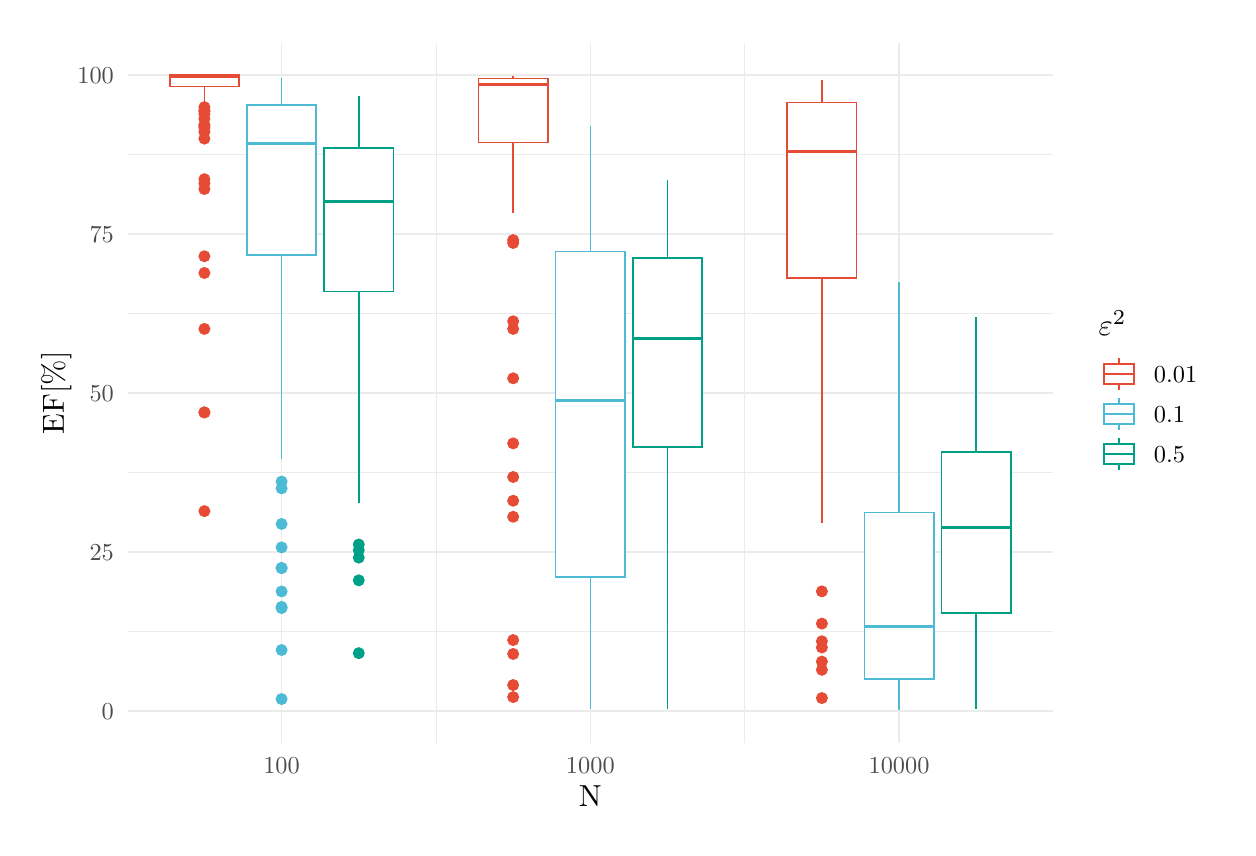
\begin{tikzpicture}[x=1pt,y=1pt]
\definecolor{fillColor}{RGB}{255,255,255}
\path[use as bounding box,fill=fillColor,fill opacity=0.00] (0,0) rectangle (433.62,289.08);
\begin{scope}
\path[clip] ( 36.11, 30.69) rectangle (370.53,283.58);
\definecolor{drawColor}{gray}{0.92}

\path[draw=drawColor,line width= 0.3pt,line join=round] ( 36.11, 70.92) --
	(370.53, 70.92);

\path[draw=drawColor,line width= 0.3pt,line join=round] ( 36.11,128.39) --
	(370.53,128.39);

\path[draw=drawColor,line width= 0.3pt,line join=round] ( 36.11,185.87) --
	(370.53,185.87);

\path[draw=drawColor,line width= 0.3pt,line join=round] ( 36.11,243.35) --
	(370.53,243.35);

\path[draw=drawColor,line width= 0.3pt,line join=round] (147.54, 30.69) --
	(147.54,283.58);

\path[draw=drawColor,line width= 0.3pt,line join=round] (259.10, 30.69) --
	(259.10,283.58);

\path[draw=drawColor,line width= 0.6pt,line join=round] ( 36.11, 42.18) --
	(370.53, 42.18);

\path[draw=drawColor,line width= 0.6pt,line join=round] ( 36.11, 99.66) --
	(370.53, 99.66);

\path[draw=drawColor,line width= 0.6pt,line join=round] ( 36.11,157.13) --
	(370.53,157.13);

\path[draw=drawColor,line width= 0.6pt,line join=round] ( 36.11,214.61) --
	(370.53,214.61);

\path[draw=drawColor,line width= 0.6pt,line join=round] ( 36.11,272.08) --
	(370.53,272.08);

\path[draw=drawColor,line width= 0.6pt,line join=round] ( 91.75, 30.69) --
	( 91.75,283.58);

\path[draw=drawColor,line width= 0.6pt,line join=round] (203.32, 30.69) --
	(203.32,283.58);

\path[draw=drawColor,line width= 0.6pt,line join=round] (314.88, 30.69) --
	(314.88,283.58);
\definecolor{drawColor}{RGB}{230,75,53}
\definecolor{fillColor}{RGB}{230,75,53}

\path[draw=drawColor,line width= 0.4pt,line join=round,line cap=round,fill=fillColor] ( 63.86,251.38) circle (  1.96);

\path[draw=drawColor,line width= 0.4pt,line join=round,line cap=round,fill=fillColor] ( 63.86,248.98) circle (  1.96);

\path[draw=drawColor,line width= 0.4pt,line join=round,line cap=round,fill=fillColor] ( 63.86,180.22) circle (  1.96);

\path[draw=drawColor,line width= 0.4pt,line join=round,line cap=round,fill=fillColor] ( 63.86,206.48) circle (  1.96);

\path[draw=drawColor,line width= 0.4pt,line join=round,line cap=round,fill=fillColor] ( 63.86,254.00) circle (  1.96);

\path[draw=drawColor,line width= 0.4pt,line join=round,line cap=round,fill=fillColor] ( 63.86,259.06) circle (  1.96);

\path[draw=drawColor,line width= 0.4pt,line join=round,line cap=round,fill=fillColor] ( 63.86,150.08) circle (  1.96);

\path[draw=drawColor,line width= 0.4pt,line join=round,line cap=round,fill=fillColor] ( 63.86,256.14) circle (  1.96);

\path[draw=drawColor,line width= 0.4pt,line join=round,line cap=round,fill=fillColor] ( 63.86,234.33) circle (  1.96);

\path[draw=drawColor,line width= 0.4pt,line join=round,line cap=round,fill=fillColor] ( 63.86,252.89) circle (  1.96);

\path[draw=drawColor,line width= 0.4pt,line join=round,line cap=round,fill=fillColor] ( 63.86,232.80) circle (  1.96);

\path[draw=drawColor,line width= 0.4pt,line join=round,line cap=round,fill=fillColor] ( 63.86,230.78) circle (  1.96);

\path[draw=drawColor,line width= 0.4pt,line join=round,line cap=round,fill=fillColor] ( 63.86,260.36) circle (  1.96);

\path[draw=drawColor,line width= 0.4pt,line join=round,line cap=round,fill=fillColor] ( 63.86,253.55) circle (  1.96);

\path[draw=drawColor,line width= 0.4pt,line join=round,line cap=round,fill=fillColor] ( 63.86,258.87) circle (  1.96);

\path[draw=drawColor,line width= 0.4pt,line join=round,line cap=round,fill=fillColor] ( 63.86,114.39) circle (  1.96);

\path[draw=drawColor,line width= 0.4pt,line join=round,line cap=round,fill=fillColor] ( 63.86,200.43) circle (  1.96);

\path[draw=drawColor,line width= 0.4pt,line join=round,line cap=round,fill=fillColor] ( 63.86,257.88) circle (  1.96);

\path[draw=drawColor,line width= 0.4pt,line join=round,line cap=round,fill=fillColor] ( 63.86,150.02) circle (  1.96);

\path[draw=drawColor,line width= 0.6pt,line join=round] ( 63.86,271.93) -- ( 63.86,272.07);

\path[draw=drawColor,line width= 0.6pt,line join=round] ( 63.86,267.84) -- ( 63.86,262.13);
\definecolor{fillColor}{RGB}{255,255,255}

\path[draw=drawColor,line width= 0.6pt,fill=fillColor] ( 51.31,271.93) --
	( 51.31,267.84) --
	( 76.41,267.84) --
	( 76.41,271.93) --
	( 51.31,271.93) --
	cycle;

\path[draw=drawColor,line width= 1.1pt] ( 51.31,271.62) -- ( 76.41,271.62);
\definecolor{drawColor}{RGB}{77,187,213}
\definecolor{fillColor}{RGB}{77,187,213}

\path[draw=drawColor,line width= 0.4pt,line join=round,line cap=round,fill=fillColor] ( 91.75,109.75) circle (  1.96);

\path[draw=drawColor,line width= 0.4pt,line join=round,line cap=round,fill=fillColor] ( 91.75, 79.34) circle (  1.96);

\path[draw=drawColor,line width= 0.4pt,line join=round,line cap=round,fill=fillColor] ( 91.75,101.28) circle (  1.96);

\path[draw=drawColor,line width= 0.4pt,line join=round,line cap=round,fill=fillColor] ( 91.75, 46.48) circle (  1.96);

\path[draw=drawColor,line width= 0.4pt,line join=round,line cap=round,fill=fillColor] ( 91.75, 64.19) circle (  1.96);

\path[draw=drawColor,line width= 0.4pt,line join=round,line cap=round,fill=fillColor] ( 91.75, 93.88) circle (  1.96);

\path[draw=drawColor,line width= 0.4pt,line join=round,line cap=round,fill=fillColor] ( 91.75, 93.76) circle (  1.96);

\path[draw=drawColor,line width= 0.4pt,line join=round,line cap=round,fill=fillColor] ( 91.75,122.61) circle (  1.96);

\path[draw=drawColor,line width= 0.4pt,line join=round,line cap=round,fill=fillColor] ( 91.75, 85.36) circle (  1.96);

\path[draw=drawColor,line width= 0.4pt,line join=round,line cap=round,fill=fillColor] ( 91.75, 79.78) circle (  1.96);

\path[draw=drawColor,line width= 0.4pt,line join=round,line cap=round,fill=fillColor] ( 91.75,125.06) circle (  1.96);

\path[draw=drawColor,line width= 0.6pt,line join=round] ( 91.75,261.10) -- ( 91.75,270.84);

\path[draw=drawColor,line width= 0.6pt,line join=round] ( 91.75,206.87) -- ( 91.75,133.20);
\definecolor{fillColor}{RGB}{255,255,255}

\path[draw=drawColor,line width= 0.6pt,fill=fillColor] ( 79.20,261.10) --
	( 79.20,206.87) --
	(104.30,206.87) --
	(104.30,261.10) --
	( 79.20,261.10) --
	cycle;

\path[draw=drawColor,line width= 1.1pt] ( 79.20,247.32) -- (104.30,247.32);
\definecolor{drawColor}{RGB}{0,160,135}
\definecolor{fillColor}{RGB}{0,160,135}

\path[draw=drawColor,line width= 0.4pt,line join=round,line cap=round,fill=fillColor] (119.64,102.33) circle (  1.96);

\path[draw=drawColor,line width= 0.4pt,line join=round,line cap=round,fill=fillColor] (119.64,100.27) circle (  1.96);

\path[draw=drawColor,line width= 0.4pt,line join=round,line cap=round,fill=fillColor] (119.64, 97.58) circle (  1.96);

\path[draw=drawColor,line width= 0.4pt,line join=round,line cap=round,fill=fillColor] (119.64, 89.37) circle (  1.96);

\path[draw=drawColor,line width= 0.4pt,line join=round,line cap=round,fill=fillColor] (119.64, 63.06) circle (  1.96);

\path[draw=drawColor,line width= 0.6pt,line join=round] (119.64,245.64) -- (119.64,264.45);

\path[draw=drawColor,line width= 0.6pt,line join=round] (119.64,193.75) -- (119.64,117.25);
\definecolor{fillColor}{RGB}{255,255,255}

\path[draw=drawColor,line width= 0.6pt,fill=fillColor] (107.09,245.64) --
	(107.09,193.75) --
	(132.20,193.75) --
	(132.20,245.64) --
	(107.09,245.64) --
	cycle;

\path[draw=drawColor,line width= 1.1pt] (107.09,226.34) -- (132.20,226.34);
\definecolor{drawColor}{RGB}{230,75,53}
\definecolor{fillColor}{RGB}{230,75,53}

\path[draw=drawColor,line width= 0.4pt,line join=round,line cap=round,fill=fillColor] (175.43,126.72) circle (  1.96);

\path[draw=drawColor,line width= 0.4pt,line join=round,line cap=round,fill=fillColor] (175.43, 62.77) circle (  1.96);

\path[draw=drawColor,line width= 0.4pt,line join=round,line cap=round,fill=fillColor] (175.43,211.28) circle (  1.96);

\path[draw=drawColor,line width= 0.4pt,line join=round,line cap=round,fill=fillColor] (175.43, 47.19) circle (  1.96);

\path[draw=drawColor,line width= 0.4pt,line join=round,line cap=round,fill=fillColor] (175.43,182.99) circle (  1.96);

\path[draw=drawColor,line width= 0.4pt,line join=round,line cap=round,fill=fillColor] (175.43,212.32) circle (  1.96);

\path[draw=drawColor,line width= 0.4pt,line join=round,line cap=round,fill=fillColor] (175.43, 51.54) circle (  1.96);

\path[draw=drawColor,line width= 0.4pt,line join=round,line cap=round,fill=fillColor] (175.43,138.87) circle (  1.96);

\path[draw=drawColor,line width= 0.4pt,line join=round,line cap=round,fill=fillColor] (175.43,180.21) circle (  1.96);

\path[draw=drawColor,line width= 0.4pt,line join=round,line cap=round,fill=fillColor] (175.43, 67.79) circle (  1.96);

\path[draw=drawColor,line width= 0.4pt,line join=round,line cap=round,fill=fillColor] (175.43,162.38) circle (  1.96);

\path[draw=drawColor,line width= 0.4pt,line join=round,line cap=round,fill=fillColor] (175.43,112.33) circle (  1.96);

\path[draw=drawColor,line width= 0.4pt,line join=round,line cap=round,fill=fillColor] (175.43,118.13) circle (  1.96);

\path[draw=drawColor,line width= 0.6pt,line join=round] (175.43,270.66) -- (175.43,271.72);

\path[draw=drawColor,line width= 0.6pt,line join=round] (175.43,247.63) -- (175.43,222.28);
\definecolor{fillColor}{RGB}{255,255,255}

\path[draw=drawColor,line width= 0.6pt,fill=fillColor] (162.88,270.66) --
	(162.88,247.63) --
	(187.98,247.63) --
	(187.98,270.66) --
	(162.88,270.66) --
	cycle;

\path[draw=drawColor,line width= 1.1pt] (162.88,268.45) -- (187.98,268.45);
\definecolor{drawColor}{RGB}{77,187,213}

\path[draw=drawColor,line width= 0.6pt,line join=round] (203.32,208.19) -- (203.32,253.54);

\path[draw=drawColor,line width= 0.6pt,line join=round] (203.32, 90.60) -- (203.32, 43.02);

\path[draw=drawColor,line width= 0.6pt,fill=fillColor] (190.77,208.19) --
	(190.77, 90.60) --
	(215.87, 90.60) --
	(215.87,208.19) --
	(190.77,208.19) --
	cycle;

\path[draw=drawColor,line width= 1.1pt] (190.77,154.31) -- (215.87,154.31);
\definecolor{drawColor}{RGB}{0,160,135}

\path[draw=drawColor,line width= 0.6pt,line join=round] (231.21,205.74) -- (231.21,233.88);

\path[draw=drawColor,line width= 0.6pt,line join=round] (231.21,137.67) -- (231.21, 42.94);

\path[draw=drawColor,line width= 0.6pt,fill=fillColor] (218.66,205.74) --
	(218.66,137.67) --
	(243.76,137.67) --
	(243.76,205.74) --
	(218.66,205.74) --
	cycle;

\path[draw=drawColor,line width= 1.1pt] (218.66,176.71) -- (243.76,176.71);
\definecolor{drawColor}{RGB}{230,75,53}
\definecolor{fillColor}{RGB}{230,75,53}

\path[draw=drawColor,line width= 0.4pt,line join=round,line cap=round,fill=fillColor] (286.99, 57.04) circle (  1.96);

\path[draw=drawColor,line width= 0.4pt,line join=round,line cap=round,fill=fillColor] (286.99, 65.12) circle (  1.96);

\path[draw=drawColor,line width= 0.4pt,line join=round,line cap=round,fill=fillColor] (286.99, 60.01) circle (  1.96);

\path[draw=drawColor,line width= 0.4pt,line join=round,line cap=round,fill=fillColor] (286.99, 85.39) circle (  1.96);

\path[draw=drawColor,line width= 0.4pt,line join=round,line cap=round,fill=fillColor] (286.99, 73.74) circle (  1.96);

\path[draw=drawColor,line width= 0.4pt,line join=round,line cap=round,fill=fillColor] (286.99, 46.83) circle (  1.96);

\path[draw=drawColor,line width= 0.4pt,line join=round,line cap=round,fill=fillColor] (286.99, 67.36) circle (  1.96);

\path[draw=drawColor,line width= 0.6pt,line join=round] (286.99,262.03) -- (286.99,270.08);

\path[draw=drawColor,line width= 0.6pt,line join=round] (286.99,198.53) -- (286.99,110.21);
\definecolor{fillColor}{RGB}{255,255,255}

\path[draw=drawColor,line width= 0.6pt,fill=fillColor] (274.44,262.03) --
	(274.44,198.53) --
	(299.54,198.53) --
	(299.54,262.03) --
	(274.44,262.03) --
	cycle;

\path[draw=drawColor,line width= 1.1pt] (274.44,244.33) -- (299.54,244.33);
\definecolor{drawColor}{RGB}{77,187,213}

\path[draw=drawColor,line width= 0.6pt,line join=round] (314.88,113.84) -- (314.88,197.09);

\path[draw=drawColor,line width= 0.6pt,line join=round] (314.88, 53.80) -- (314.88, 42.37);

\path[draw=drawColor,line width= 0.6pt,fill=fillColor] (302.33,113.84) --
	(302.33, 53.80) --
	(327.43, 53.80) --
	(327.43,113.84) --
	(302.33,113.84) --
	cycle;

\path[draw=drawColor,line width= 1.1pt] (302.33, 72.66) -- (327.43, 72.66);
\definecolor{drawColor}{RGB}{0,160,135}

\path[draw=drawColor,line width= 0.6pt,line join=round] (342.77,135.84) -- (342.77,184.37);

\path[draw=drawColor,line width= 0.6pt,line join=round] (342.77, 77.54) -- (342.77, 42.91);

\path[draw=drawColor,line width= 0.6pt,fill=fillColor] (330.22,135.84) --
	(330.22, 77.54) --
	(355.32, 77.54) --
	(355.32,135.84) --
	(330.22,135.84) --
	cycle;

\path[draw=drawColor,line width= 1.1pt] (330.22,108.44) -- (355.32,108.44);
\end{scope}
\begin{scope}
\path[clip] (  0.00,  0.00) rectangle (433.62,289.08);
\definecolor{drawColor}{gray}{0.30}

\node[text=drawColor,anchor=base east,inner sep=0pt, outer sep=0pt, scale=  0.88] at ( 31.16, 39.15) {0};

\node[text=drawColor,anchor=base east,inner sep=0pt, outer sep=0pt, scale=  0.88] at ( 31.16, 96.63) {25};

\node[text=drawColor,anchor=base east,inner sep=0pt, outer sep=0pt, scale=  0.88] at ( 31.16,154.10) {50};

\node[text=drawColor,anchor=base east,inner sep=0pt, outer sep=0pt, scale=  0.88] at ( 31.16,211.58) {75};

\node[text=drawColor,anchor=base east,inner sep=0pt, outer sep=0pt, scale=  0.88] at ( 31.16,269.05) {100};
\end{scope}
\begin{scope}
\path[clip] (  0.00,  0.00) rectangle (433.62,289.08);
\definecolor{drawColor}{gray}{0.30}

\node[text=drawColor,anchor=base,inner sep=0pt, outer sep=0pt, scale=  0.88] at ( 91.75, 19.68) {100};

\node[text=drawColor,anchor=base,inner sep=0pt, outer sep=0pt, scale=  0.88] at (203.32, 19.68) {1000};

\node[text=drawColor,anchor=base,inner sep=0pt, outer sep=0pt, scale=  0.88] at (314.88, 19.68) {10000};
\end{scope}
\begin{scope}
\path[clip] (  0.00,  0.00) rectangle (433.62,289.08);
\definecolor{drawColor}{RGB}{0,0,0}

\node[text=drawColor,anchor=base,inner sep=0pt, outer sep=0pt, scale=  1.10] at (203.32,  7.64) {N};
\end{scope}
\begin{scope}
\path[clip] (  0.00,  0.00) rectangle (433.62,289.08);
\definecolor{drawColor}{RGB}{0,0,0}

\node[text=drawColor,rotate= 90.00,anchor=base,inner sep=0pt, outer sep=0pt, scale=  1.10] at ( 13.08,157.13) {EF[\%]};
\end{scope}
\begin{scope}
\path[clip] (  0.00,  0.00) rectangle (433.62,289.08);
\definecolor{drawColor}{RGB}{0,0,0}

\node[text=drawColor,anchor=base west,inner sep=0pt, outer sep=0pt, scale=  1.10] at (387.03,177.78) {$\varepsilon^2$};
\end{scope}
\begin{scope}
\path[clip] (  0.00,  0.00) rectangle (433.62,289.08);
\definecolor{drawColor}{RGB}{230,75,53}

\path[draw=drawColor,line width= 0.6pt] (394.25,158.20) --
	(394.25,160.37);

\path[draw=drawColor,line width= 0.6pt] (394.25,167.59) --
	(394.25,169.76);
\definecolor{fillColor}{RGB}{255,255,255}

\path[draw=drawColor,line width= 0.6pt,fill=fillColor] (388.83,160.37) rectangle (399.67,167.59);

\path[draw=drawColor,line width= 0.6pt] (388.83,163.98) --
	(399.67,163.98);
\end{scope}
\begin{scope}
\path[clip] (  0.00,  0.00) rectangle (433.62,289.08);
\definecolor{drawColor}{RGB}{77,187,213}

\path[draw=drawColor,line width= 0.6pt] (394.25,143.74) --
	(394.25,145.91);

\path[draw=drawColor,line width= 0.6pt] (394.25,153.14) --
	(394.25,155.31);
\definecolor{fillColor}{RGB}{255,255,255}

\path[draw=drawColor,line width= 0.6pt,fill=fillColor] (388.83,145.91) rectangle (399.67,153.14);

\path[draw=drawColor,line width= 0.6pt] (388.83,149.53) --
	(399.67,149.53);
\end{scope}
\begin{scope}
\path[clip] (  0.00,  0.00) rectangle (433.62,289.08);
\definecolor{drawColor}{RGB}{0,160,135}

\path[draw=drawColor,line width= 0.6pt] (394.25,129.29) --
	(394.25,131.46);

\path[draw=drawColor,line width= 0.6pt] (394.25,138.69) --
	(394.25,140.85);
\definecolor{fillColor}{RGB}{255,255,255}

\path[draw=drawColor,line width= 0.6pt,fill=fillColor] (388.83,131.46) rectangle (399.67,138.69);

\path[draw=drawColor,line width= 0.6pt] (388.83,135.07) --
	(399.67,135.07);
\end{scope}
\begin{scope}
\path[clip] (  0.00,  0.00) rectangle (433.62,289.08);
\definecolor{drawColor}{RGB}{0,0,0}

\node[text=drawColor,anchor=base west,inner sep=0pt, outer sep=0pt, scale=  0.88] at (406.98,160.95) {0.01};
\end{scope}
\begin{scope}
\path[clip] (  0.00,  0.00) rectangle (433.62,289.08);
\definecolor{drawColor}{RGB}{0,0,0}

\node[text=drawColor,anchor=base west,inner sep=0pt, outer sep=0pt, scale=  0.88] at (406.98,146.50) {0.1};
\end{scope}
\begin{scope}
\path[clip] (  0.00,  0.00) rectangle (433.62,289.08);
\definecolor{drawColor}{RGB}{0,0,0}

\node[text=drawColor,anchor=base west,inner sep=0pt, outer sep=0pt, scale=  0.88] at (406.98,132.04) {0.5};
\end{scope}
\end{tikzpicture}
%
        }
        \caption{Empirical \acrshort{ef} for the setup of \Cref{ex:ess_failure} for varying sample sizes $N$ and $\varepsilon^{2}$ and $M=100$ replications. Here $\G = \mathcal N(0,1)$ and $\P = \frac{1}{2} \left( \mathcal N (0,1) + \mathcal N(0, \varepsilon^{-2}) \right)$. In all scenarios the second moment $\rho$ is infinite, thus high \acrshortpl{ef} are misleading us to believe that importance sampling performs well when it does not.}
        \label{fig:ess_failure}
    \end{figure}

\end{example}

As an alternative, we may want to assess whether importance sampling has converged through the empirical variance of $\hat \zeta_{N}$,\footnote{As the following arguments depend on the sample size $N$, we mark this dependency by adding $N$ to the subscript of the estimator.} i.e., 
$$
\widehat\var \left( \hat\zeta_{N} \right) = \frac{1}{N}\left(\frac{1}{N} \sum_{i = 1}^N w_{i}^{2} f(X^{i})^{2} - \hat \zeta_{N}^{2}\right)
$$
is, while seemingly natural, flawed \citep{Chatterjee2018Sample}.
Indeed, the authors show that for any given threshold $\epsilon$ we may find an $N$ which only depends on $\epsilon$, such that the probability that the empirical variance exceeds $\epsilon$ for this $N$ is small. This is summarized in the following theorem.

\begin{theorem}[{\cite[Theorem 2.1]{Chatterjee2018Sample}}]
    \label{thm:variance_failure}
    Given any $\epsilon > 0$, there exists $N \leq \epsilon^{-2} 2^{1 + \epsilon^{-3}}$ such that the following is true. Take any $\G$ and $\P$ as in \Cref{thm:chatterje2018Thm1}, and any $f: \mathcal X \to \R$ such that $ \lVert f \rVert_{L^{2}(\P)} \leq 1.$ Then 
    $$
        \mathbb P \left( \widehat \var \left( \hat \zeta_{N} \right) < \epsilon\right) \geq 1 - 4 \epsilon.
    $$
\end{theorem}

The problem here is that $N$ does not depend on $\G$ and $\P$, so we may choose $\G$ almost singular to $\P$. As an example, take $\P = \mathcal N(0, 1)$ and $\G = \mathcal N(0, \sigma^{2})$ for $\sigma^{2} > \frac{1}{2}$. The weights are then given by $$w(x) = \sigma \exp \left( - \frac{x^{2}}{2} \left( 1 - \frac{1}{\sigma^{2}} \right) \right),$$
and for $X \sim \G$ the variance of $w(X)X$ is 
\begin{align}
    \label{eq:variance-wxx}
\tau^{2} = \var \left( w(X)X \right) = \frac{\sigma^{4}}{\left( 2 \sigma^{2} - 1 \right)^{\frac{3}{2}}}
\end{align}
which goes to $\infty$ as $\sigma^2$ does, see the appendix for details. Thus, for a pre-specified $\epsilon > 0$, let $N$ be as in \Cref{thm:variance_failure} and choose $\sigma^{2}$ such that $\var \left( \hat\zeta_{N} \right) = \frac {\tau^{2}}N$ is larger than, say, $10\epsilon$. By the preceding theorem, we would, with large probability, observe a small empirical variance and thus declare $\hat\zeta_{N}$ to have converged, whereas, in reality, we would need a sample size that is $100$ times as large.

Thus using the empirical variance as a threshold for convergence should be avoided, at least for importance sampling where the weights can be evaluated exactly. For self-normalized importance sampling, the authors do not provide such a theorem. As a remedy \citep{Chatterjee2018Sample} suggest the heuristic $q_{N} = \mathbb E Q_{N}$ where
$$
Q_{N} = \max_{1\leq i\leq N} W_{i} \in [0, 1].
$$
This judges whether importance sampling has collapsed to just a few particles and is itself amenable to Monte-Carlo integration, by repeatedly sampling $N$ samples from $\G$ and calculating the weights. 
As this requires multiple runs of importance sampling, it may, however, be prohibitively expensive in practice.

In the following sections, we will predominantly take the position that we are interested in finding a good particle approximation $\hat\P_{N}$ of the form \Cref{eq:is-particle-approximation} over finding the optimal proposal $\G^{\ast}$ from \Cref{prop:minimum_MSE_IS} and assume that the importance sampling weights can only be evaluated up to a constant. 
This has several reasons: First of all, for most problems considered in this thesis $\P$ is usually a conditional distribution, e.g. $\P = \mathbb P^{X|Y=y}$ for states $X$ and observations $Y$ in the \acrshort{ssm} context. Should the appropriate densities exist, evaluating the weights amounts to calculating 
$$
\rnd{\mathbb P^{X| Y= y}}{\G}(x) = \frac{p(x|y)}{g(x)} = \frac{p(y|x)p(x)}{g(x)p(y)} \propto \frac{p(y|x)p(x)}{g(x)}.
$$
In these situations $p(y) = \int p(x,y)\d x$ is usually intractable. For $\G^{\ast}$ we are in the same situation, where the evaluation of the integration constant $\P \lvert f \rvert$ is infeasible, but the density $\lvert f(x)\rvert p(x)$ is available.
% do not focus on a single f
Second, focusing on the particle approximation allows us to consider multiple test functions $f$, e.g. focus on different marginals of $\P$, which is usually what practitioners are interested in. 
%Third, for maximum likelihood estimation (\Cref{sec:maximum_likelihood_estimation}), we will see that these two notions coincide.
% simplify notation: P always target, G always proposal
Finally, this allows us to simplify the notation used in this thesis. $\P$ will always be the probability measure of interest and $\G$ the proposal. In later parts of this thesis, we will predominantly perform Gaussian importance sampling, i.e. $\G = \mathcal N(\mu, \Sigma)$, hence a handy mnemonic is to think of $\G$ as a \textbf{G}aussian proposal.

Let us now turn towards the problem of finding a good proposal $\G$ for a given $\P$. 

\subsection{\texorpdfstring{\Acrfull{la}}{Laplace approximation}}
\label{subsec:la}

The \acrfull{la} goes back to Laplace \citep{Laplace1986Memoir} who invented the technique to approximate moments of otherwise intractable distributions. Since \citep{Tierney1986Accurate,Tierney1989Fully} rediscovered its use to approximate posterior means and variances, it has been a staple method for approximate inference.
The method is based on a second-order Taylor series expansion of the log target density $\log p(x)$ around its mode $\hat x$, i.e. matching mode and curvature. Assuming the density is sufficiently smooth, we have
\begin{align}
    \label{eq:LA_approximation}
\log p(x) \approx \log p(\hat x) + \underbrace{\nabla_{x} \log p (\hat x)}_{= 0} \left( x - \hat x \right) + \frac{1}{2} (x - \hat x)^{T} H (x - \hat x)
\end{align}
where $H$ is the Hessian of $\log p$ evaluated at $\hat x$. As $\log p (\hat x)$ does not depend on $x$, the right-hand side can be seen (up to additive constants) as the density of a Gaussian distribution with mean $\hat x$ and covariance matrix $\Sigma = - H^{-1}$. Thus using $\G = \mathcal N (\hat x, -H^{-1})$ as a proposal in importance sampling seems promising. 
% degenerate case when $H$ is not PSD
If $\hat x$ is the unique global mode of $p$ and $H$ is negative definite, the \gls{la} yields an actual Gaussian distribution. 
% numerics
To obtain the \acrshort{la} in practice, a Newton-Raphson scheme may be used, which conveniently tracks $H$ as well. Furthermore, if $\P$ includes more structure, e.g. it is the smoothing density in the \acrshort{ssm} context, we may be able to exploit this structure to design efficient Newton-Raphson schemes, see \Cref{subsec:glssm-approach}.

% advantages / disadvantages
The main advantage of the \gls{la} is that it is usually fast to obtain and, for sufficiently well-behaved distributions on a moderate dimensional space, provides reasonably high \gls{ess}. Additionally, the Newton-Raphson iterations to find the mode and Hessian are robust and require no simulation, unlike the other methods discussed further below.
For the \glspl{ssm} we consider in this thesis, the numerical methods can be implemented using the Kalman filter and smoother \citep{Shephard1997Likelihood,Durbin1997Monte}, even in the degenerate case where $H$ is indefinite \citep{Jungbacker2007Monte}, see also \Cref{subsec:glssm-approach}.

However, as the \gls{la} is a local approximation, it may be an inappropriate description of the global behavior of the target, see \Cref{ex:la_failure} for a breakdown of \gls{la}, and the simulation studies presented in \Cref{sec:simulation_studies}. 
Additionally, even if the \gls{la} works in principle, its \gls{ess} will usually degenerate quickly once the dimension increases whereas the \gls{cem} and \gls{eis} do so at a slower pace.

%\glsreset{vm}
\subsection{\texorpdfstring{\Acrfull{vmm}}{Variance Minimization method}}
As we have discussed above, the second moment 
$$
\rho = \G [w^{2}]
$$
plays an important role in the performance of importance sampling. Naturally, we may want to choose $\G$ such that $\rho$ becomes minimal. To this end we consider tractable, parametric proposals $\left( \G_{\psi} \right)_{\psi \in \Psi}$ for a parameter set $\Psi$, where usually $\Psi \subseteq \R^{k}$. Noticing that $\G_{\psi} w_{\psi} = 1$, we see that minimizing $\rho_{\psi} = \G_{\psi}[w^{2}_\psi]$ over $\Psi$ is equivalent to minimizing
$$
\var \left( w_{\psi}(X_{\psi}) \right) = \G_{\psi}[w_{\psi}^2] - \G_{\psi}[w_{\psi}]^{2} = \rho_{\psi} - 1,
$$
over $\Psi$ where $X_{\psi} \sim \G_{\psi}$. This is the \gls{vmm} 
\glsreset{cem}
\subsection{The \texorpdfstring{\Acrfull{cem}}{Cross-Entropy method}}
\label{subsec:cem}
Recall from our discussion surrounding \Cref{thm:chatterje2018Thm1} that for importance sampling to be effective, we should have a small \acrshort{kld} between the target $\P$ and the proposal $\G$. As the \acrshort{kld} depends on global properties, i.e. the Radon-Nikodym derivative $\rnd{\P}{\G}$, minimizing it should lead to a global approximation of $\P$, improving on the local-approximation provided by the \acrshort{la}.

The \gls{cem}\citep{Rubinstein1999CrossEntropy,Rubinstein2004CrossEntropy} implements this idea and selects from a parametric family $ \left( \G_{\psi} \right)_{\psi \in \Psi}$ of proposals the one that minimizes the \gls{kld} to the target. Here $\Psi$ is usually a subset of $\R^{k}$. We will usually assume the existence of a common dominating measure $\mu$ for both $\P$ and all $\G_{\psi}$, $\psi \in \Psi$ with corresponding densities $p$ and $g_{\psi}$, $\psi \in \Psi$. The importance sampling weights are then given by 
$$
w_{\psi}(x) = \frac{p(x)}{g_{\psi}(x)},
$$
$x \in \mathcal X$, or, if either on of $p$ and $g_\psi$ is only available up to a constant, by 
$$
\tilde w_{\psi} (x) \propto \frac{p(x)}{g_{\psi}(x)}.
$$
If the dependence on $\psi$ is not of interest or the particular $\psi$ is obvious from the context, we may drop the subscript. 

The \acrshort{cem} finds $\psi_{\text{CE}}$ which solves the following optimization problem
\begin{align*}
    \psi_{\text{CE}} &= \argmin_{\psi \in \Psi} \Dkl{\P}{\G_{\psi}} \\
    &= \argmin_{\psi \in \Psi} \P \left[ \log w_{\psi}\right]
\end{align*}
The existence and uniqueness of $\psi_{\text{CE}}$ will depend heavily on the choice of parametric family $(\G_{\psi})_{\psi \in \Psi}$ and $\P$. 

If $\P$ and $\G_{\psi}$ possess densities $p$ and $g_{\psi}$ w.r.t. some common measure $\mu$, the same for all $\psi$, we may reformulate the optimization problem to maximize the cross-entropy between $p$ and $g_{\psi}$ instead:
\begin{align}
    \begin{split}
    \psi_{\text{CE}} &= \argmin_{\psi \in \Psi} \P \left[\log p \right] - \P \left[\log g_{\psi}\right] \\
    &= \argmax_{\psi \in \Psi} \P \left[\log g_{\psi}\right]
    \end{split} \label{eq:ce_argmax}.
\end{align}
Suppose now that $\psi \mapsto \log g_{\psi}(x)$ is (strictly) concave for $\P$-almost every $x \in \mathcal X$ and $\Psi$ is a convex subset of $\R^{k}$. Then $\psi \mapsto \P \left[\log g_{\psi}\right]$ is (strictly) concave as well. As a consequence, we may apply the usual results from convex optimization, i.e. every local maximum is a global one, the set of maximizers is convex and if $\psi \mapsto \log g_{\psi}(x)$ is strictly convex for $\P$-almost every $x$, there is at most one maximizer \todo{ref}.

As we have seen in \Cref{lem:log-concavity}, the densities of exponential families are log-concave in the natural parameter, and as such they will be the ideal candidates for our investigations. 

%\begin{theorem}[consistencty of $\hat\psi_{\text{CE}}$]
%    \label{thm:ce-m-estimator}
%    Assume the following technical conditions apply:
%    \begin{itemize}
%        \item[A1] Uniform consistency of importance sampling
%            $$\sup_{\psi \in \Psi}\lVert \hat \G_N (w\log g_\psi) - \G(w \log g_\psi) \rVert \stackrel{P}{\to} 0$$ 
%        \item[A2] Regularity condition
%            $$ \partial_\psi \P \left(\log g_\theta\right) = \P \left(\partial_\theta \log g_\theta\right) $$
%            for all $\psi \in \Psi$
%        \item[A3] positive definite misspecified Fisher information
%            $$ \P \left(\left(\partial_\psi \log g_\theta\right)\left(\partial_\theta \log g_\theta\right)^T\right) > 0$$
%    \end{itemize}
%
%    Then $\hat\psi_{\text{CE}}$ is a consistent estimator of $\psi_{\text{CE}}$.
%\end{theorem}
%
%\begin{theorem}[asymptotic normality of $\hat\psi_{\text{CE}}$]
%    
%\end{theorem}

% analytical solution, MLE
An additional attractive property of the \gls{cem} for exponential families with natural parameter $\psi \in \R^{k}$, the optimal $\psi_{\text{CE}}$ only depends on the expected value $\P [T]$. 

\begin{proposition}[The \acrshort{cem} for exponential families]
    \label{prop:cem_exponential_families}
    Let $\left( \G_{\psi} \right)_{\psi \in \Psi}$ form a $k$-dimensional natural exponential family with log-densities 
    $$
    \log g_{\psi}(x) = \log h(x) + \psi^{T} T(x) - \log Z(\psi),
    $$
    and convex parameter space $\Psi \subseteq \R^{k}$. 
    Suppose $T, \log (h) \in L^{1}(\P)$.

    If there is a $\psi$ such that 
    $$
    \P[T] = \G_{\psi} [T],
    $$
    then $\psi = \pce$ is a maximizer of \Cref{eq:ce_argmax}. If $\cov_{\G_{\psi}} T$ is positive definite for all $\psi\in\Psi$, then the maximizer is unique.
\end{proposition}

\begin{proof}
    The target may be rewritten as
    $$
    \psi \mapsto f(\psi) = \P \left[\log g_{\psi}(x)\right]= \P [\log h] - \log Z(\psi) + \psi^{T} \P [T].
    $$
    As $\log Z(\psi)$ is the cumulant-generating function of $\G_{\psi}$ it is twice differentiable, and so is $f$. The gradient of $\log Z(\psi)$ is 
    $$
    \nabla_{\psi} \log Z(\psi) = \G_{\psi} T
    $$
    and its Hessian is 
    $$
    H_{\psi} \log Z(\psi) = \cov_{\G_{\psi}} T
    $$
    the covariance of $T$ under $\G_{\psi}$. Thus the Hessian of $f$ is 
    $$
    H_{\psi} f = - \cov_{\G_{\psi}} T,
    $$
    which is negative-semi-definite. Thus $f$ is concave, and any local maximizer $\psi$ is a global maximizer. The gradient of $f$ is 
    $$
        \nabla_{\psi} f(\psi) = \P[T] - \G_{\psi} [T],
    $$
    thus the optimal $\psi_{\text{CE}}$ solves
    $$
    \P[T] = \G_{\pce}[T].
    $$
    If $\cov_{\G_{\psi}} T$ is positive definite for all $\psi \in \Psi$, $f$ is strictly concave, and the maximizer is unique.
\end{proof}
As a consequence, the \acrshort{cem} for natural exponential families reduces to matching the moments of the sufficient statistic of the target and proposal.
In many cases, this system of equations can be solved analytically or by gradient descent algorithms.
Let us discuss the assumptions and applicability of this proposition. Assuming that $T, \log h \in L^{1}(\P)$ is necessary for the target to be finite, so it cannot be dropped. The proof of uniqueness relies on $\cov_{\G_{\psi}} T$ being positive definite, to ensure that $\psi \mapsto \log Z(\psi)$ is strictly convex. This could also be achieved by requiring the exponential family to be minimal, see \citep[Theorem 1.13 (iv)]{Brown1986Fundamentals}. The existence of a $\psi$ such that $\P T = \G_{\psi} T$ is not restrictive for most commonly used distributions: for the (multivariate) normal, Poisson, negative binomial and binomial distribution there is always a unique solution, as the sufficient statistics consist of means and covariances. 

While $\P T$ is usually not available, it is itself amenable to importance sampling. Given a proposal $\G$ we may estimate $\P T$ by $\hat\P_N T = \sum_{i = 1}^{N} W^{i} T(X^{i})$ for $X^{1}, \dots, X^{N} \iid \G$ and auto-normalized importance sampling weights $W^{i}$ and in turn, applying \Cref{prop:cem_exponential_families}, estimate $\psi_{\text{CE}}$ by $\hat \psi_{\text{CE}}$ solving
$$
\hat \P_N T = \G_{\hpce} T.
$$
As $T, \log h \in L^{1}(\hat \P_{N})$, the only conditions we have to check to apply the above proposition is that this equation has a unique solution and that $\Psi$ is convex. 

In what follows, we will derive novel results on the performance of this estimator. In particular, we will investigate under which conditions $\hpce$ is consistent and asymptotically normal. While we restrict ourselves here to the setting of $k$-dimensional natural exponential families, these results should generalize to other classes of distributions as well. The advantage that this class of families has is that due to the structure of the densities, they provide straightforward (regularity) conditions for the asymptotic results to hold.

% proof: appeal to vdV, pd ensures that M(\theta) is convex, so global maximum unique and well separated
$\hat\psi_{\text{CE}}$ is a Z-estimator, i.e. an estimator that arises from solving a random system of equations, and we can analyze its asymptotic behavior using standard results from the theory of Z-estimators. 
The following theorem of \citep{VanderVaart2000Asymptotic} will be useful in analyzing the asymptotic behavior of the estimators we consider in this thesis. We state it here, using our notation, for completeness.

\begin{theorem}[asymptotic normality of Z-estimators, {\citep[Theorem 5.21]{VanderVaart2000Asymptotic}}]
    \label{thm:clt_z_est_vdv}
    For every $\psi$ in an open subset of $\R^{k}$, let $x \mapsto f_{\psi}(x)$ be a measurable vector-valued function such that, for every $\psi_{1}$ and $\psi_{2}$ in a neighborhood of $\psi_{0}$ and a measurable function $\dot f$ with $\G \left[\dot f\right] < \infty$,
    \begin{align}
    \label{eq:clt-vdv-local-lipschitz}
    \lVert f_{\psi_{1}}(x) - f_{\psi_{2}}(x)\rVert \leq \dot f(x) \lVert \psi_{1} - \psi_{2}\rVert \tag{LL}.
    \end{align}

    Assume that $\G \left[\lVert f_{\psi_{0}}\rVert \right] < \infty$ and that the map $\psi \mapsto \G \left[f_{\psi}\right]$ is differentiable at $\psi_{0}$, with nonsingular derivative matrix $B^{-1}$. Let $X_{1}, \dots, X_{N} \iid \G$ and $\hat \G_{N} = \sum_{i = 1}^{N} \delta_{X^{i}}$. If $\hat\psi_{N}$ fulfills $$\hat\G_{N} \left[f_{\hat\psi_{N}}\right] = o_{P} \left( N^{-\frac{1}{2}} \right),$$ and $\hat\psi_{N} \to \psi_{0}$ in probability, then
    \begin{align}
        \label{eq:clt-vdv}
        \sqrt{N} \left( \hat\psi_{N} - \psi_{0} \right) \Dto \mathcal N(0, BMB^{T}),
    \end{align}
    where $M = \G f_{\psi_{0}} f_{\psi_{0}}^{T}$.
\end{theorem}

\begin{notation}[central limit theorem for Z-estimators]
    \label{not:notation-clt}
    The central limit theorems derived in this and the next section will make frequent use of \Cref{thm:clt_z_est_vdv}. We will use the following consistent notation in the statement of theorems and their proofs:
    \begin{itemize}
        \item $f_\psi(x): \R^{k} \to \R^{k}$ the estimating equation              
        \item $B = \left(\G\partial_{\psi} f_{\psi}\right)^{-1}$ the bread matrix
        \item $M = \G f_{\psi}f_{\psi}^{T}$ the meat matrix
        \item $V = BMB$ the asymptotic covariance matrix
        \item $\log g_{\psi}(x) = \psi^{T}T(x) + \log h(x) - \log Z(\psi)$ the density of the natural exponential family considered
        \item $\dot z (\psi) = \nabla_{\psi}\log Z(\psi) = \G_{\psi} T$ the derivative of the log-normalizing constant $\psi \mapsto \log Z(\psi)$
        \item $\ddot z(\psi) = \partial_{\psi} \dot z(\psi) =\cov_{\G_{\psi}}T$ the Hessian of the log-normalizing constant $\psi \mapsto \log Z(\psi)$
    \end{itemize}
    The naming of $B$ and $M$ stems from the sandwich estimator \citep{White1982Maximum}, where the bread $B$ is the Jacobian of the estimating equations $\P f_{\psi} = 0$ and the meat $M$ is the covariance matrix of $f_{\psi}$ under $\P$, thus making a \glqq{}meat sandwich\grqq{}.
\end{notation}

\todo{discussion on relevance and novelty of these results}
\begin{theorem}[consistency of $\hat \psi_{\text{CE}}$]
    \label{thm:ce-consistent}
    \todo{from van der Vaart/Casella Berger}
\end{theorem}


\begin{theorem}[asymptotic normality of $\hat \psi_{\text{CE}}$]
    \label{thm:ce-clt}
    %\todo{require unique solution?}
    Let $\G_{\psi}$ form a natural exponential family with densities $g_{\psi}(x) = \frac{h(x)}{Z(\psi)} \exp \left( \psi^{T}T(x)\right) $ w.r.t. $\mu$. Let $\G, \P$ be two other probability measures such that $\G \ll \P$ and let $W = \frac{\d \P}{\d \G}$ be the normalized importance sampling weights. 
    Suppose further that 
    \begin{enumerate}[label={\bfseries(A{\arabic*})}]
        \item\label{it:exist-unique-psice} $\G_{\hpce} T = \hat\P_{N} T$ $\mu$-a.s. has a unique solution $\hpce$,
        \item\label{it:zdot-ll} $\psi \mapsto \nabla_\psi \log Z(\psi)$ is locally Lipschitz around $\psi_{\text{CE}}$,
        \item\label{it:w-t-wt-L2} $W,T$ and $WT$ possess finite second moments  w.r.t. $\G$,
        \item\label{it:FI-psd} the Fisher information $I(\psi_{\text{CE}})$ is positive definite and equal to $-\ddot z(\pce)$, additionally $\psi \mapsto I(\psi)$ is continuous, and
        \item\label{it:ce-regularity} the regularity conditions of \Cref{thm:ce-consistent} hold.
    \end{enumerate}

    Then, as $N$ goes to $\infty$,
    $$
        \sqrt{N} \left(\hat\psi_\text{CE} - \psi_{\text{CE}}\right) \Dto \mathcal N \left(0, V_{\text{CE}}\right)
    $$
    where 
    $$
    V_{\text{CE}} = B_\ce M_\ce B_\ce,%I(\psi_{\text{CE}})^{-1}  \text{Cov}_{\G} \left( W (T - \G_{\pce}T) \right) I(\psi_{\text{CE}})^{-1},
    $$
    with 
    \begin{align*}
        B_{\ce} &= I(\pce)^{-1}, \\
        M_{\ce} &= \cov_{\G} \left( W (T - \G_{\pce}T) \right).
    \end{align*}
    Moreover $\G (W(T - \G_{\pce}T))) = 0$, so we may estimate $V_{\text{CE}}$ consistently by plug-in:
    $$
    \hat V_{\text{CE}} = I(\hat\psi_{\text{CE}})^{-1}  \left(\sum_{i = 1}^N W^{2}_{i} \left(T(X^{i}) - \G_{\hpce}T \right)\left(T(X^{i}) - \G_{\hpce} T\right)^{T} \right)I(\hat\psi_{\text{CE}})^{-1}.
    $$
\end{theorem}

\begin{proof} We check that the conditions of the central limit theorem for Z-estimators (\Cref{thm:clt_z_est_vdv}) are fulfilled. This proof uses the notation established in \Cref{not:notation-clt}. Consider the estimating equations for $\pce$ 
    $$x\mapsto f_\psi(x) = \nabla_{\psi} \left(w(x)\log g_{\psi}(x)\right) = w(x) T(x) - w(x) \dot z (\psi),$$ where $w(x)$ are the unnormalized importance sampling weights. 
    By \ref{it:exist-unique-psice} $\hat \P_{N} f_{\hpce} = 0$ $\mu$-a.s., so it remains to show that $\hpce \to \pce$  in probability, which is implied by \Cref{thm:ce-consistent}.
    
    As $$\left\lVert f_{\psi_1}(x) - f_{\psi_2}(x)\right\rVert = w(x) \left\lVert \dot z (\psi_1) - \dot z(\psi_2)\right\rVert$$ for all $\psi_{1}, \psi_{2}\in \Psi$,  $\G w < \infty $ and \ref{it:zdot-ll} imply the local Lipschitz condition \Cref{eq:clt-vdv-local-lipschitz} in \Cref{thm:clt_z_est_vdv}.
    Furthermore, by \ref{it:w-t-wt-L2} it holds
    %\todo{fix: no triangle equation (squared norm)}
    $$
    \G \left\lVert f_\psi \right\rVert^2 \leq \G w^2 \left\lVert \dot z(\psi) \right\rVert ^2  + 2 \lVert \dot z(\psi) \rVert \G \lVert wT\rVert + \G \left\lVert wT\right\rVert^2 < \infty.
    $$

    Additionally $\psi \mapsto\G f_\psi = (\G w) \dot z (\psi) + \G wT$ is differentiable everywhere, with Jacobian $(\G w) \ddot z(\psi)$, where  $\ddot z(\psi) = \partial_\psi \dot z(\psi)$ is the Hessian of the cumulant generating function, which equals the negative Fisher information $-I(\pce)$ as $\G_{\psi}, \psi \in \Psi$ form a natural exponential family and the regularity conditions \ref{it:ce-regularity} allow differentiation under the integral.
    Thus we see that 
    $$
    \G f_{\pce} = \P \left( \dot z(\pce) + T \right) = \dot z (\pce) + \P T = 0,
    $$
    by definition of $\pce$, so $$\text{Cov}_{\G} \left( w(T - \nabla_{\pce} \log Z (\pce)) \right) = \text{Cov}_{\G}(f_{\pce}) = \G f_{\pce}f_{\pce}^{T}.$$
    As $W = \frac{w}{\G w}$
    By \Cref{eq:clt-vdv} the asymptotic covariance matrix is 
    $$
    V_{\ce} = B_{\ce}M_{\ce}B_{\ce}
    $$
    which shows the asymptotic normality. 

    Estimating $B_{\ce}$ by $\hat B_{\ce}= I(\hpce)$ and $$M_{\ce} = \G W^{2} (T - \G_{\pce}T)(T - \G_{\pce}T)^{T} = \P W (T - \G_{\pce})(T - \G_{\pce})^T$$ by $$\hat M_{\ce} = \hat\P_{N} W \left( T - \G_{\hpce} T \right)\left( T - \G_{\hpce} T \right)^{T}$$
    yields the stated plug-in estimator. 
    The promised consistency follows from \ref{it:w-t-wt-L2} and \ref{it:FI-psd}.
\end{proof}

The form of the asymptotic covariance matrix is that of the sandwich estimator \citep{White1982Maximum}, corrected for the importance sampling with $\G$. This is not surprising: the \acrshort{cem} essentially performs maximum likelihood estimation of $\psi$ where the data come from the misspecified $\P$. Additionally, we have to correct the variance for performing importance sampling with $\G$, instead of sampling directly from $\P$.

As mentioned above, if $(\G_\psi)_{\psi \in \Psi}$ do not form an exponential family, $\hat\psi_{\text{CE}}$ will still be consistent and asymptotically normal, provided the usual regularity conditions for M-estimators, or Z-estimators if $\log g_{\psi}$ is sufficiently smooth, apply. 

% break-down in higher dimensions?

% iterative procedure, CRNs

% applications of CEM
The \gls{cem} is routinely used for estimating failure probabilities for rare events \citep{Homem-de-Mello2007Study} and has been applied to Bayesian inference \citep{Engel2023Bayesian,Ehre2023Certified} and optimal control problems \citep{Kappen2016Adaptive,Zhang2014Applications}.
\todo{more lit. review CEM}

\glsreset{eis}
\subsection{\texorpdfstring{\Acrfull{eis}}{Efficient importance sampling}}
\label{subsec:eis}
\gls{eis} \citep{Richard2007Efficient} provides an alternative to the \gls{cem}. Instead of minimizing the \gls{kld} between the target $\P$ and proposal $\G_{\psi}, \psi \in \Psi$, \gls{eis} aims at minimizing the variance of the logarithm of importance sampling weights. 
Our discussion of \citep{Chatterjee2018Sample}, \Cref{thm:chatterje2018Thm1}, especially \Cref{lem:bounded-log-variance}, suggests that this is worthwhile. 
Thus, \acrshort{eis} finds $\peis$ which is a feasible solution to the following optimization problem
\begin{align}
    \label{eq:eis_optim}
\min_{\psi \in \Psi} \text{Var}_{\P} \left[ \log w_{\psi} \right] = \min_{\psi \in \Psi} \P \left[ \log w_{\psi} - \P \log w_{\psi} \right]^{2},
\end{align}
where, as in the last section, $\log w_{\psi} = \log p - \log g_{\psi}$.

Two problems arise: $\P [\log w_{\psi}] = \Dkl{\P}{\G_{\psi}}$ is usually intractable and we usually only have access to the unnormalized weights $\frac{\tilde w_{\psi}}{\G_{\psi} \left[ w_{\psi} \right]} = w_{\psi}$, with unknown integration constant $\G_{\psi} \left[ w_{\psi} \right]$. Both can be dealt with by introducing the nuisance parameter $\lambda = \P \left[ \log \tilde w_{\psi} \right]$, utilizing the fact that the mean is the minimizer of the squared distance functional with the minimum value equal to the variance, should it exist. Indeed 
$$
    \log w_{\psi} - \P [\log w_{\psi}] = \log \tilde w_{\psi} - \log \G_{\psi} [\tilde w_{\psi}] - \P \left[ \log \tilde w_{\psi} \right] + \log \G_{\psi}[\tilde w_{\psi}] = \log \tilde w_{\psi} - \P \left[ \log \tilde w_{\psi} \right],
$$
so
$$
    \min_{\psi \in \Psi} \P \left[ \log w_{\psi} - \P \left[ \log w_{\psi} \right] \right]^{2} = \min_{\psi \in \Psi, \lambda \in \R} \P \left[ \log \tilde w_{\psi} - \lambda \right]^{2},
$$
where $\psi\in \Psi$ is a minimizer of the left-hand side if, and only if, $(\psi, \lambda) \in \Psi \times \R$ with $\lambda = \P \left[ \log \tilde w_{\psi} \right]$ is a minimizer of the right-hand side. 

Similar to the \gls{cem} we restrict our in-depth analysis to natural exponential family proposals where $$\log g_{\psi}(x) = \psi^{T}T(x) - \log Z(\psi).$$ In this case the optimization problem is reduced to
\begin{align}
    \label{eq:eis_exponential_families}
    \min_{\psi \in \Psi, \lambda \in \R} \P \left[ \log p - \psi^{T}T - \lambda \right]^{2},
\end{align}
a weighted linear least squares problem. As we consider unnormalized weights $\tilde w$, we are additionally able to get rid of the potentially non-linear term $\log Z(\psi)$.
Noticing that this is a convex objective function in $\psi$ which, similar to the \acrshort{cem}, will be very useful to derive asymptotics later on. For now, we begin with studying the existence and uniqueness of $\peis$ similar to \Cref{prop:cem_exponential_families}.

\begin{lemma}[\acrshort{eis} for exponential families]
    \label{prop:eis_exponential_families}
    Let $\left( \G_{\psi} \right)_{\psi \in \Psi}$ form a k-dimensional natural exponential family with log-densities 
    $$
        \log g_{\psi}(x) = \psi^{T} T(x) - \log Z(\psi)
    $$
    for $\Psi \subseteq \R^{k}$. Suppose that $\log p, T \in L^{2}(\P)$. 

    If there is a $\peis \in \Psi$ with
    \begin{align}
        \label{eq:peis-analytical}
        \cov_{\P} \left( T \right)\peis = \cov_{\P} \left(T, \log p \right)
    \end{align}
    it is a global minimizer of \Cref{eq:eis_optim}. If $\cov_{\P} \left( T \right)$ is non-singular,
    $$
    \peis = \cov_{\P} (T) ^{-1} \cov _{\P} (T, \log p )
    $$
    is the unique global minimizer.
\end{lemma}

\begin{proof}
    Under the proposed conditions, we may consider \Cref{eq:eis_exponential_families} instead, where the moment conditions on $\log p $ and $T$ ensure that the problem is well-posed, i.e. the target is finite for all $\psi \in \Psi$. 
    Thus the optimal $ \left( \peis, \lambda_{\eis} \right)$ are given by the \gls{blup} of $\log p $ by the sufficient statistic $T$ under $\P$ for $\peis$ and $\P \left[ \log \tilde w_{\peis} \right]$ for $\lambda_{\eis}$. Standard results from multivariate regression theory imply that the \acrshort{blup} is given by any solution of
    $$
        \cov_{\P} (T) \peis = \cov_{\P} (T, \log p),
    $$
    i.e. $\peis$ as stated in the lemma. Furthermore, if $\cov_{\P} (T)$ is non-singular, the solution to this equation is unique.
    
\end{proof}

As the optimal $\peis$ depends on several unknown quantities, \gls{eis} proceeds like the \gls{cem} and employs importance sampling with a proposal $\G$, estimating $\peis$ by
$$
\left(\hat \lambda,\hat \psi_{\text{EIS}}\right) = \argmin_{\lambda,\psi} \hat\P_{N} \left[ \log \tilde w_{\psi} - \lambda \right]
$$
where $X^{1}, \dots, X^{N} \iid \G$. 
Again, if $\G_{\psi}, \psi \in \Psi$ form an exponential family with natural parameter $\psi$, this optimization problem turns into a weighted least squares problem, so we can estimate $\peis$ with the standard weighted least squares estimator
$$
\left( \hat\lambda', \hpeis \right) = \left(\mathbf X^{T}\mathbf W\mathbf X\right)^{-1}\mathbf X^{T}\mathbf W y%
$$
where the random design matrix $\mathbf X$\footnote{if $\mathbf X\mathbf W \mathbf X$ is not invertible, replace the inverse by the Moore-Penrose pseudoinverse} and diagonal weights matrix $\mathbf W$ are given by
\begin{align*}
\mathbf X &= \begin{pmatrix}
    1 & T(X^{1})^{T} \\
    \dots&\dots\\
    1 & T(X^{N})^{T} \\
\end{pmatrix}\\
\intertext{and}
\mathbf W &= \text{diag} \left( W^{1}, \dots, W^{N} \right),
\end{align*}
and the observations are 
\begin{align*}
y = \left( \log p(X^{1}), \dots, \log p(X^{N}) \right)^{T} \in \R^{N}.
\end{align*}

Alternatively, replacing $\P$ by $\hat\P_{N}$ in \Cref{eq:peis-analytical}, we obtain the equivalent formulation
\begin{align}
    \label{eq:hpeis-cov}
    \hpeis = \cov_{\hat\P_{N}} (T)^{-1} \cov_{\hat \P_{N}} \left( T, \log p \right),
\end{align}
as long as $\cov_{\hat \P_{N}} T$ is non-singular.

An attractive feature of \gls{eis} is that if the target $\P$ is a member of the exponential family of proposals, i.e. there is a $\psi_{\P}\in\Psi$ such that $\P = \G_{\psi_{\P}}$, then \gls{eis} finds the optimal $\peis = \psi_{\P}$ a.s. for a finite number of samples.

\begin{proposition}[Finite sample convergence of \gls{eis}]
    \label{prop:eis-finite-sample}
    Suppose $\G_{\psi}, \psi \in \Psi \subseteq \R^{k}$ for a natural exponential family w.r.t. Lebesgue measure, where the support of the sufficient statistic $\operatorname{supp} T$ is open in $\R^{k}$. 
    Furthermore let $\G$ be a probability measure on $\R^{m}$ that is equivalent to $\P$, i.e. $\G \ll \P$ and $\P \ll \G$. 

    If there is a $\psi_{\P} \in \Psi$ such that $\P = \G_{\psi_{\P}}$, then $\hpeis = \psi_{\P}$ a.s. for $N \geq k$. 
\end{proposition}

\begin{proof}
   As $\P$ stems from the same exponential family as $\G_{\psi}$, the pseudo-observations are $$\log p  = \psi_{\P}^T T - \log Z(\psi_{\P}).$$ Thus $\cov_{\hat \P_{N}} \left( T, \log p  \right) = \cov_{\hat \P_{N}} \left( T \right)\psi_{\P}$. 
   If we can show that $\cov_{\hat\P_{N}} T$ is non-singular, \Cref{eq:hpeis-cov} implies that $\hpeis = \psi_{\P}$ a.s.. 

   If $\cov_{\hat \P_{N}} T$ were singular, there would exist a $\psi \in \R^{k}$ such that
   $$
   \psi^{T} \cov_{\hat\P_{N}} (T) \psi = \cov_{\hat \P_{N}} \left( \psi^{T}T \right) = 0.
   $$
    In this case the a.s. non-zero $W^{i}(X^{i}) T(X^{i})$ would lie in the orthogonal complement $\psi^{\perp}$ for all $i = 1, \dots, N$. As the weights are a.s. positive by the assumed equivalence of $\G$ and $\P$, the same holds true for $T(X^{i}), i = 1,\dots, N$.
   If $N$ is bigger than $k$, the probability that this happens is $0$, as $\operatorname{supp} T $ is open. Thus $\cov_{\hat \P_{N}} T$ is non-singular almost surely and the result is shown.
\end{proof}

Note that if in the above proposition only $\G_{\psi} \gg \P$ holds, we obtain, by a similar argument, that $$\mathbb P \left( \hpeis = \psi_{\P} \right) \stackrel{N\to\infty}\longrightarrow 1.$$
Additionally, we then have to take care of the event $ \{ w(X) = 0 \}$, whose probability is now potentially positive.

We now turn to deriving asymptotics for $\hpeis$. As for the \acrshort{cem}, we start with proving that $\hpeis$ consistently estimates $\peis$.
For this we need to ensure that $\peis$ is the unique solution to \Cref{eq:eis_optim}, as otherwise, consistent estimators of $\peis$ cannot exist. 
As \Cref{eq:eis_exponential_families} is a linear least squares problem, the objective function is convex, and so we can apply \Cref{thm:haberman-consistent} and \Cref{prop:is-consistency}.

\begin{theorem}[consistency of $\hpeis$]
    \label{thm:eis-consistent}
    Let $\left( \G_{\psi} \right)_{\psi \in \Psi}$ form a $k$-dimensional natural exponential family with log-densities 
    $$
        \log g_{\psi}(x) = \psi^{T}T(x) - \log Z(\psi)
    $$
    for convex $\Psi \subseteq \R^{k}$. Let $\G \gg \P$ be a proposal and suppose that 
    \begin{enumerate}
        \item $\log p, T \in L^{2}(\P)$ and
        \item $\cov_\P (T)$ is non-singular,
        \item $\peis \in \operatorname{int} \Psi.$ 
    \end{enumerate}
    
    Then 
    $$
        \hpeis \stackrel{N \to \infty}\longrightarrow \peis
    $$
    almost surely.
\end{theorem}

\begin{proof}
    We follow the same strategy as in the proof of \Cref{thm:cem-consistent}. Let 
    \begin{align*}
        b: \R^{p} \times \R^{k + 1} \to [-\infty, \infty)  && b(x,\psi') = \begin{cases}
            -\frac{1}{2} \left( \log p(x) - \psi^{T}T(x) - \lambda \right)^{2} & \psi \in \Psi \\
            -\infty &  \text{ else,}
        \end{cases}
    \end{align*}
    where $\psi' = (\psi, \lambda) \in \R^{k + 1}$. For fixed $x$ this function is concave, as its Hessian is negative semi-definite:
    $$
        H_{\psi'} b(x, \psi') = -\begin{pmatrix}
            1 & T(x)^{T} \\
            T(x) & T(x)T(x)^{T}
        \end{pmatrix} = -\begin{pmatrix} 1 & T(x)^{T} \end{pmatrix} \begin{pmatrix} 1 & T(x)^{T} \end{pmatrix}^{T},
    $$
    if $\psi \in \Psi$. Let $X^{1}, \dots, X^{N} \iid \P$ and let $\tilde \P _{N}$ be their empirical distribution. For $\psi \in \Psi, \lambda \in \R$ we have 
    $$
        \P \left[ b(\cdot, \psi') \right] = - \frac{1}{2} \P \left[ \left( \log p - \psi^{T}T - \lambda\right)^{2} \right] < \infty,
    $$
    as $\log p, T\in L^{2}(\P)$. Let us now check that conditions \ref{it:C1} - \ref{it:C3} are fulfilled. 

    \ref{it:C1} is fulfilled, as we assumed $\peis \in \operatorname{int} \Psi$. \ref{it:C2} holds, as $\peis$ is the unique global maximizer by \Cref{prop:eis_exponential_families}, as $\cov (T)$ is non-singular.
    \ref{it:C3} obviously holds. 

    Thus $\hpeis$ is strongly consistent if $\G = \P$. If $\G$ is different from $\P$, we can apply \Cref{prop:is-consistency}, where the existence of M-estimators is ensured by \Cref{eq:hpeis-cov}, using the Moore-Penrose inverse if $\cov_{\hat\P_{N}}(T)$ is singular. 
\end{proof}

As \Cref{eq:hpeis-cov} expresses $\hpeis$ in terms of empirical covariances, we could alternatively prove consistency by ensuring that the empirical covariances are consistent as well, for which we would need to ensure that fourth-order moments of $\log p$ and $T$ w.r.t. $\P$ exist. This strategy may be fruitful if $\peis$ does not lie in the interior of $\Psi$, although the more sophisticated treatment of \citep{Haberman1989Concavity} may also be applicable under these circumstances.

Additionally, if fourth-order moments exist, we can derive a central limit theorem, similar to \Cref{thm:cem-clt}, for \acrshort{eis}.

% region CLT proof
\begin{theorem}[\acrshort{clt} for $\hpeis$]
    \label{thm:eis-clt}
    Let $\left( \G_{\psi} \right)_{\psi \in \Psi}$ form a $k$-dimensional natural exponential family with log-densities 
    $$
    \log g_{\psi}(x) = \psi^{T} T(x) - \log Z(\psi),
    $$
    and convex parameter space $\Psi \subseteq \R^{k}$. Let $\G \gg \P$ be a proposal with weights $w = \rnd{\P}{\G}$. 

    Assume that
    \begin{enumerate}
        \item\label{it:secondISmomentsexist}$w T_{i}T_{j}, w (\log p)^{2} \in L^{2}(\G)$ for $i,j = 1, \dots, k$,
        \item\label{it:fourthmomentsexist} $\log p, T_i \in L^{4}(\P)$ for all $i = 1, \dots, k$
        \item $\cov_{\P}(T)$ is non-singular and $\peis \in \operatorname{int} \Psi$.
    \end{enumerate}

    Then 
    $$
        \sqrt{N} (\hpeis - \peis) \convD \Normal (0, BMB)
    $$
    where $B = \cov_{\P}(T)^{-1}$ and 
    $$
    M = \cov_{\G} \left( w \left( \log p - \peis^{T}T - \lambda_{\eis} - \P[T] \right)T \right).
    $$
\end{theorem}

\begin{proof}
    Similar to the proof of \Cref{thm:cem-clt}, we combine \Cref{thm:haberman-clt} and \Cref{prop:is-clt}. Let 
    \begin{align*}
        b : \mathcal X \times \R^{k + 1} \to [-\infty, \infty) && b(x, \psi') =  \begin{cases}
            -\frac{1}{2} \left( \log p(x) - \psi^{\prime T}T'(x) \right) & x \in \Psi \\
            -\infty & \text{else,}
        \end{cases}
    \end{align*}
    where $\psi' = (\psi, \lambda) \in \Psi \times\R$ and $T'(x) = \begin{pmatrix} T(x) & 1 \end{pmatrix}$. For $\psi \in \Psi$ the map $(\psi, \lambda) \to \P [b(\cdot, (\psi, \lambda))]$ is differentiable with gradient 
    $$
        \nabla_{\psi'} \P [b(\cdot, \psi')] = - \P \left[\left( \log p - \psi^{\prime T}T' \right) T'\right] = \begin{pmatrix}
            - \P \left[ T'\log p - T'T^{\prime T}\psi' \right] \\
            -\P \left[ \log p - \psi'^{T}T' \right]
        \end{pmatrix}
    $$
    and Hessian 
    $$
        H_{\psi'} \P[b(\cdot, \psi')] = -\P\left[T'T^{\prime T}\right] = - \begin{pmatrix}
            \P \left[ TT^{T} \right] & \P [T^{T}] \\
            \P [T] & 1
        \end{pmatrix}.
    $$
    The Hessian is negative definite, as for all $\psi\in \R^{k}, \lambda \in \R$ we have
    \begin{align*}
        \begin{pmatrix} \psi^{T} & \lambda \end{pmatrix} H_{\psi'} \P \left[ b(\cdot, \psi') \right]\begin{pmatrix} \psi^{T} & \lambda \end{pmatrix}^{T} &= - \left( \psi^{T} \cov_{\P} (T) \psi + \psi^{T}\P[T]\P[T]^{T}\psi + 2 \psi^{T}\P[T] \lambda + \lambda^{2}\right) \\
                                 &= - \left( \psi^{T}\cov_{\P}(T)\psi + (\lambda + \psi^{T}\P[T])^{2} \right) \leq 0,
    \end{align*}
    with equality if, and only if, both $\lambda$ and $\psi$ are $0$, as $\cov_{\P}(T)$ is assumed to be positive definite. Thus condition \ref{it:C7} is fulfilled.

    For condition \ref{it:C10}, we can verify that for all $i,j = 1,\dots, k+ 1$ 
    $$
        (\nabla_{\psi'} b(\cdot, \psi'))_{i}(\nabla_{\psi'} b(\cdot, \psi'))_{j} = \left( \log p - \psi^{\prime T}T' \right)^{2} T'_{i}T'_{j}
    $$
    is in $L^{1}(\P)$ by assumption \ref{it:fourthmomentsexist} and the Hölder inequality. 

    To apply \Cref{prop:is-clt} we need to show that $w(\cdot)b'(\cdot, \psi',\xi') \in L^{2}(\G)$ for all $\xi'\in\R^{k + 1}$ and all $\psi'$ in a neighborhood of $\peis$, for this it suffices that we show 
    $$
        w^{2}(\nabla_{\psi'} b(\cdot, \psi'))_{i}(\nabla_{\psi'} b(\cdot, \psi'))_{j} = w^{2}\left( \log p - \psi^{\prime T}T' \right)^{2} T'_{i}T'_{j}
    $$
    is in $L^{1}(\G)$, which holds, again, by assumption \Cref{it:secondISmomentsexist} and the Hölder inequality.

    We have thus shown a central limit theorem for $\hat\psi'_{\eis} = \left( \hpeis, \hat\lambda_{\eis} \right)$, i.e. 
    $$
        \sqrt{N} \left( \hat\psi'_{\eis} - \peis \right) \to \mathcal N(0, M'B'M')
    $$
    with $B' = - \left(H_{\psi'_{\eis}} \P \left[ b(\cdot, \psi'_{\eis}) \right]\right)^{-1}$ and $M' = \cov \left( w(X) \nabla_{\psi'_{\eis}} b(X,\psi'_{\eis}) \right)$ for $X \sim \G$. By using the inversion formula for block matrices, we obtain 
    \begin{align*}
        B' &= \begin{pmatrix}
            \P \left[ TT^{T} \right] & \P [T^{T}] \\
            \P [T] & 1
        \end{pmatrix}^{-1} = \begin{pmatrix}
            \Sigma + \mu\mu^{T} & \mu^{T} \\
            \mu & 1
        \end{pmatrix}^{-1} \\
        &= \begin{pmatrix}
            (\Sigma + \mu\mu^{T} - \mu\mu^{T})^{-1} & 0 \\
            0 & 1 - \mu^{T} (\Sigma + \mu\mu^{T})^{-1}\mu
        \end{pmatrix} \begin{pmatrix}
            I_{k} & - \mu^{T} \\
            -\mu(\Sigma + \mu\mu^{T})^{-1}& 1
        \end{pmatrix} \\
        &= \begin{pmatrix}
            \Sigma^{-1} & - \mu^{T}\Sigma^{-1}\\
            -\Sigma^{-1}\mu& 1 - \mu^{T} \left( \Sigma + \mu\mu^{T} \right)^{-1}\mu
        \end{pmatrix}
    \end{align*}
    where $\Sigma = \cov_{\P} (T)$ and $\mu = \P [T]$. Similarly, 
    $$
        M' = \begin{pmatrix}
            \cov_{\G} \left( w W_{\peis}T \right) &\cov_{\G} \left( w W_{\peis}T, w W_{\peis} \right) \\
            \cov_{\G} \left( w W_{\peis}, w W_{\peis}T \right) & \cov_{\G} \left( w W_{\peis} \right) 
        \end{pmatrix},
    $$
    where $W_{\peis} = \log p - \psi^{\prime T}_{\eis}T'$.

    If $\mu \neq 0$, we may change the sufficient statistic of the exponential family such that this holds, i.e. let $\tilde T = T - \P [T]$, then 
    $$
        \log g_{\psi}(x) = \psi^{T}T(x) - \log Z(\psi) = \psi^{T}\tilde T(x) - \log \tilde Z(\psi)
    $$
    where $\tilde Z(\psi) = \log Z(\psi) + \P [T]$. As $\peis$, \Cref{eq:peis-analytical}, only depends on $T - \P[T]$ under $\P$, this does not change $\peis$. Similarly, $\hpeis$, \Cref{eq:hpeis-cov}, is unaffected by subtracting a constant from $T$. Only 
    $$
        \tilde \lambda_{\eis} = \lambda_{\eis} + \P[T]
    $$
    and similarly $\hat\lambda_{\eis}$ are changed.
    
    Thus, without loss of generality, we may assume that $\P[T] = 0$. 
    Then 
    $$
        B' = \begin{pmatrix}
            \Sigma^{-1} & 0 \\
            0 & 1
        \end{pmatrix}
    $$
    is a diagonal matrix. Taking the $\peis$ marginal of the asymptotic normal distribution, we arrive at 
    $$
        \sqrt{N} \left( \hpeis - \peis \right) \to \mathcal N \left( 0, BMB \right)
    $$
    with $B = \cov_{\P}(T)$ and $M = \cov_{G} \left( w \left( \log p - \peis^{T}T - \lambda_{\eis} - \P[T] \right)T \right)$, as promised.
    
\end{proof}
% endregion 


A discussion of the assumptions of \Cref{thm:eis-consistent,thm:eis-clt} is in order. We start with the consistency result \Cref{thm:eis-consistent}. The integrability condition, i.e that $\log p, T \in L^{2}(\P)$ is necessary to ensure existence of $\peis$ and the existence of $\cov_{\P}(T)$ as well as $\peis \in \operatorname{int} \Psi$ ensure uniqueness, see also \Cref{prop:eis_exponential_families}. 

Regarding the central limit theorem \Cref{thm:eis-clt}, requiring the existence of higher order moments is natural. Unfortunately, there is no direct interpretation of these requirements as generalizations of the existence of $\rho$, as was the case for the \acrshort{cem}. 

The only integrability conditions related to the proposal $\G$ are those for $wT_{i}T_{j}$ and $w \log(p)^{2}$. 
Choosing $\left(\G_{\psi}\right)_{\psi \in \Psi}$ to consist of Gaussian distributions, the conditions on $T$ translate to the existence of certain polynomial moments of $w^{2}$ w.r.t. the proposal $\G$ (or $w$ w.r.t. $\P$). This technical condition, is not easily interpreted, as assuming existence of moments of the target distribution seem more natural than those involving the extra weighting term $w = \frac{p}{g}$, which depends on the proposal $\G$ as well. 